% Options for packages loaded elsewhere
\PassOptionsToPackage{unicode}{hyperref}
\PassOptionsToPackage{hyphens}{url}
\PassOptionsToPackage{dvipsnames,svgnames,x11names}{xcolor}
%
\documentclass[
  11pt,
]{krantz}
\usepackage{amsmath,amssymb}
\usepackage{lmodern}
\usepackage{iftex}
\ifPDFTeX
  \usepackage[T1]{fontenc}
  \usepackage[utf8]{inputenc}
  \usepackage{textcomp} % provide euro and other symbols
\else % if luatex or xetex
  \usepackage{unicode-math}
  \defaultfontfeatures{Scale=MatchLowercase}
  \defaultfontfeatures[\rmfamily]{Ligatures=TeX,Scale=1}
  \setmonofont[Scale=0.775]{MesloLGS NF}
\fi
% Use upquote if available, for straight quotes in verbatim environments
\IfFileExists{upquote.sty}{\usepackage{upquote}}{}
\IfFileExists{microtype.sty}{% use microtype if available
  \usepackage[]{microtype}
  \UseMicrotypeSet[protrusion]{basicmath} % disable protrusion for tt fonts
}{}
\makeatletter
\@ifundefined{KOMAClassName}{% if non-KOMA class
  \IfFileExists{parskip.sty}{%
    \usepackage{parskip}
  }{% else
    \setlength{\parindent}{0pt}
    \setlength{\parskip}{6pt plus 2pt minus 1pt}}
}{% if KOMA class
  \KOMAoptions{parskip=half}}
\makeatother
\usepackage{xcolor}
\IfFileExists{xurl.sty}{\usepackage{xurl}}{} % add URL line breaks if available
\IfFileExists{bookmark.sty}{\usepackage{bookmark}}{\usepackage{hyperref}}
\hypersetup{
  pdftitle={Appunti di Costruzione e validazione di strumenti di misura dell'efficacia dell'intervento psicologico in neuropsicologia -- B020881 (B213)},
  pdfauthor={Corrado Caudek},
  colorlinks=true,
  linkcolor={Maroon},
  filecolor={Maroon},
  citecolor={Blue},
  urlcolor={Blue},
  pdfcreator={LaTeX via pandoc}}
\urlstyle{same} % disable monospaced font for URLs
\usepackage{color}
\usepackage{fancyvrb}
\newcommand{\VerbBar}{|}
\newcommand{\VERB}{\Verb[commandchars=\\\{\}]}
\DefineVerbatimEnvironment{Highlighting}{Verbatim}{commandchars=\\\{\}}
% Add ',fontsize=\small' for more characters per line
\usepackage{framed}
\definecolor{shadecolor}{RGB}{248,248,248}
\newenvironment{Shaded}{\begin{snugshade}}{\end{snugshade}}
\newcommand{\AlertTok}[1]{\textcolor[rgb]{0.33,0.33,0.33}{#1}}
\newcommand{\AnnotationTok}[1]{\textcolor[rgb]{0.37,0.37,0.37}{\textbf{\textit{#1}}}}
\newcommand{\AttributeTok}[1]{\textcolor[rgb]{0.61,0.61,0.61}{#1}}
\newcommand{\BaseNTok}[1]{\textcolor[rgb]{0.06,0.06,0.06}{#1}}
\newcommand{\BuiltInTok}[1]{#1}
\newcommand{\CharTok}[1]{\textcolor[rgb]{0.5,0.5,0.5}{#1}}
\newcommand{\CommentTok}[1]{\textcolor[rgb]{0.37,0.37,0.37}{\textit{#1}}}
\newcommand{\CommentVarTok}[1]{\textcolor[rgb]{0.37,0.37,0.37}{\textbf{\textit{#1}}}}
\newcommand{\ConstantTok}[1]{\textcolor[rgb]{0,0,0}{#1}}
\newcommand{\ControlFlowTok}[1]{\textcolor[rgb]{0.27,0.27,0.27}{\textbf{#1}}}
\newcommand{\DataTypeTok}[1]{\textcolor[rgb]{0.27,0.27,0.27}{#1}}
\newcommand{\DecValTok}[1]{\textcolor[rgb]{0.06,0.06,0.06}{#1}}
\newcommand{\DocumentationTok}[1]{\textcolor[rgb]{0.37,0.37,0.37}{\textbf{\textit{#1}}}}
\newcommand{\ErrorTok}[1]{\textcolor[rgb]{0.14,0.14,0.14}{\textbf{#1}}}
\newcommand{\ExtensionTok}[1]{#1}
\newcommand{\FloatTok}[1]{\textcolor[rgb]{0.06,0.06,0.06}{#1}}
\newcommand{\FunctionTok}[1]{\textcolor[rgb]{0,0,0}{#1}}
\newcommand{\ImportTok}[1]{#1}
\newcommand{\InformationTok}[1]{\textcolor[rgb]{0.37,0.37,0.37}{\textbf{\textit{#1}}}}
\newcommand{\KeywordTok}[1]{\textcolor[rgb]{0.27,0.27,0.27}{\textbf{#1}}}
\newcommand{\NormalTok}[1]{#1}
\newcommand{\OperatorTok}[1]{\textcolor[rgb]{0.43,0.43,0.43}{\textbf{#1}}}
\newcommand{\OtherTok}[1]{\textcolor[rgb]{0.37,0.37,0.37}{#1}}
\newcommand{\PreprocessorTok}[1]{\textcolor[rgb]{0.37,0.37,0.37}{\textit{#1}}}
\newcommand{\RegionMarkerTok}[1]{#1}
\newcommand{\SpecialCharTok}[1]{\textcolor[rgb]{0,0,0}{#1}}
\newcommand{\SpecialStringTok}[1]{\textcolor[rgb]{0.5,0.5,0.5}{#1}}
\newcommand{\StringTok}[1]{\textcolor[rgb]{0.5,0.5,0.5}{#1}}
\newcommand{\VariableTok}[1]{\textcolor[rgb]{0,0,0}{#1}}
\newcommand{\VerbatimStringTok}[1]{\textcolor[rgb]{0.5,0.5,0.5}{#1}}
\newcommand{\WarningTok}[1]{\textcolor[rgb]{0.37,0.37,0.37}{\textbf{\textit{#1}}}}
\usepackage{longtable,booktabs,array}
\usepackage{calc} % for calculating minipage widths
% Correct order of tables after \paragraph or \subparagraph
\usepackage{etoolbox}
\makeatletter
\patchcmd\longtable{\par}{\if@noskipsec\mbox{}\fi\par}{}{}
\makeatother
% Allow footnotes in longtable head/foot
\IfFileExists{footnotehyper.sty}{\usepackage{footnotehyper}}{\usepackage{footnote}}
\makesavenoteenv{longtable}
\usepackage{graphicx}
\makeatletter
\def\maxwidth{\ifdim\Gin@nat@width>\linewidth\linewidth\else\Gin@nat@width\fi}
\def\maxheight{\ifdim\Gin@nat@height>\textheight\textheight\else\Gin@nat@height\fi}
\makeatother
% Scale images if necessary, so that they will not overflow the page
% margins by default, and it is still possible to overwrite the defaults
% using explicit options in \includegraphics[width, height, ...]{}
\setkeys{Gin}{width=\maxwidth,height=\maxheight,keepaspectratio}
% Set default figure placement to htbp
\makeatletter
\def\fps@figure{htbp}
\makeatother
\setlength{\emergencystretch}{3em} % prevent overfull lines
\providecommand{\tightlist}{%
  \setlength{\itemsep}{0pt}\setlength{\parskip}{0pt}}
\setcounter{secnumdepth}{5}
\usepackage{amsmath}
\usepackage{amssymb}
\usepackage{amsfonts}

\defaultfontfeatures{Scale=MatchLowercase}

\usepackage{booktabs}
\usepackage{longtable}
\usepackage[bf,singlelinecheck=off]{caption}

\usepackage{framed,color}
\definecolor{shadecolor}{RGB}{248,248,248}

\renewcommand{\textfraction}{0.05}
\renewcommand{\topfraction}{0.8}
\renewcommand{\bottomfraction}{0.8}
\renewcommand{\floatpagefraction}{0.75}

\renewenvironment{quote}{\begin{VF}}{\end{VF}}
\let\oldhref\href
\renewcommand{\href}[2]{#2\footnote{\url{#1}}}

\ifxetex
  \usepackage{letltxmacro}
  \setlength{\XeTeXLinkMargin}{1pt}
  \LetLtxMacro\SavedIncludeGraphics\includegraphics
  \def\includegraphics#1#{% #1 catches optional stuff (star/opt. arg.)
    \IncludeGraphicsAux{#1}%
  }%
  \newcommand*{\IncludeGraphicsAux}[2]{%
    \XeTeXLinkBox{%
      \SavedIncludeGraphics#1{#2}%
    }%
  }%
\fi

\makeatletter
\newenvironment{kframe}{%
\medskip{}
\setlength{\fboxsep}{.8em}
 \def\at@end@of@kframe{}%
 \ifinner\ifhmode%
  \def\at@end@of@kframe{\end{minipage}}%
  \begin{minipage}{\columnwidth}%
 \fi\fi%
 \def\FrameCommand##1{\hskip\@totalleftmargin \hskip-\fboxsep
 \colorbox{shadecolor}{##1}\hskip-\fboxsep
     % There is no \\@totalrightmargin, so:
     \hskip-\linewidth \hskip-\@totalleftmargin \hskip\columnwidth}%
 \MakeFramed {\advance\hsize-\width
   \@totalleftmargin\z@ \linewidth\hsize
   \@setminipage}}%
 {\par\unskip\endMakeFramed%
 \at@end@of@kframe}
\makeatother

\renewenvironment{Shaded}{\begin{kframe}}{\end{kframe}}

\usepackage{makeidx}
\makeindex

\urlstyle{tt}

\usepackage{amsthm}
\makeatletter
\def\thm@space@setup{%
  \thm@preskip=8pt plus 2pt minus 4pt
  \thm@postskip=\thm@preskip
}
\makeatother

\DeclareMathOperator{\V}{\mathbb{V}} % Define variance operator
\DeclareMathOperator{\Var}{\mathbb{V}} % Define variance operator
\DeclareMathOperator{\SD}{SD} % Define sd operator
\DeclareMathOperator{\Cov}{Cov} % Define covariance operator
\DeclareMathOperator{\Corr}{Corr} % Define correlation operator
\DeclareMathOperator{\Me}{Me} % Define mediane operator
\DeclareMathOperator{\Mo}{Mo} % Define mode operator

\DeclareMathOperator{\Bin}{Binomial} % Define binomial operator
\DeclareMathOperator{\Bernoulli}{Bernoulli} % Define Bernoulli operator
\DeclareMathOperator{\Ber}{\mathscr{B}} % Define Bernoulli operator
\DeclareMathOperator{\Poi}{Poisson} % Define Poisson operator
\DeclareMathOperator{\Uniform}{Uniform} % Define Uniform operator
\DeclareMathOperator{\Cauchy}{Cauchy} % Define Cauchy operator
\DeclareMathOperator{\B}{B} % beta function
% \mbox{B}(a, b) % beta function
% \mbox{Beta}(a, b) % beta distribution

\DeclareMathOperator{\elpd}{elpd} % Define elpd operator
\DeclareMathOperator{\lppd}{lppd} % Define lppd operator
\DeclareMathOperator{\LOO}{LOO} % Define LOO operator
\DeclareMathOperator{\argmin}{arg\,min} 
\DeclareMathOperator{\argmax}{arg\,max} 

\newcommand{\E}{\mathbb{E}} % Define expected value operator
\newcommand{\R}{\textsf{R}} % Define R programming language symbol
\newcommand{\Real}{\mathbb{R}} % Define real number operator
\newcommand{\Prob}{\mathscr{P}}
\newcommand{\indep}{\perp \!\!\! \perp}

\usepackage[
 labelfont=bf,
 font={small, it}
]{caption}
\usepackage{upquote} % print correct quotes in verbatim-environments
\usepackage{empheq}
\usepackage{xfrac}

\usepackage{polyglossia}
\setmainlanguage{italian}

\frontmatter
\usepackage{booktabs}
\usepackage{longtable}
\usepackage{array}
\usepackage{multirow}
\usepackage{wrapfig}
\usepackage{float}
\usepackage{colortbl}
\usepackage{pdflscape}
\usepackage{tabu}
\usepackage{threeparttable}
\usepackage{threeparttablex}
\usepackage[normalem]{ulem}
\usepackage{makecell}
\usepackage{xcolor}
\ifLuaTeX
  \usepackage{selnolig}  % disable illegal ligatures
\fi
\usepackage[]{natbib}
\bibliographystyle{apalike}

\title{Appunti di Costruzione e validazione di strumenti di misura dell'efficacia dell'intervento psicologico in neuropsicologia -- B020881 (B213)}
\author{Corrado Caudek}
\date{2022-03-03}

\begin{document}
\maketitle

\cleardoublepage\newpage\thispagestyle{empty}\null
% \cleardoublepage\newpage\thispagestyle{empty}\null
%\cleardoublepage\newpage
\thispagestyle{empty}
\begin{center}
\Large{Appunti di Costruzione e validazione di strumenti di misura dell'efficacia dell'intervento psicologico in neuropsicologia -- AA 2021/2022}

\vskip20pt

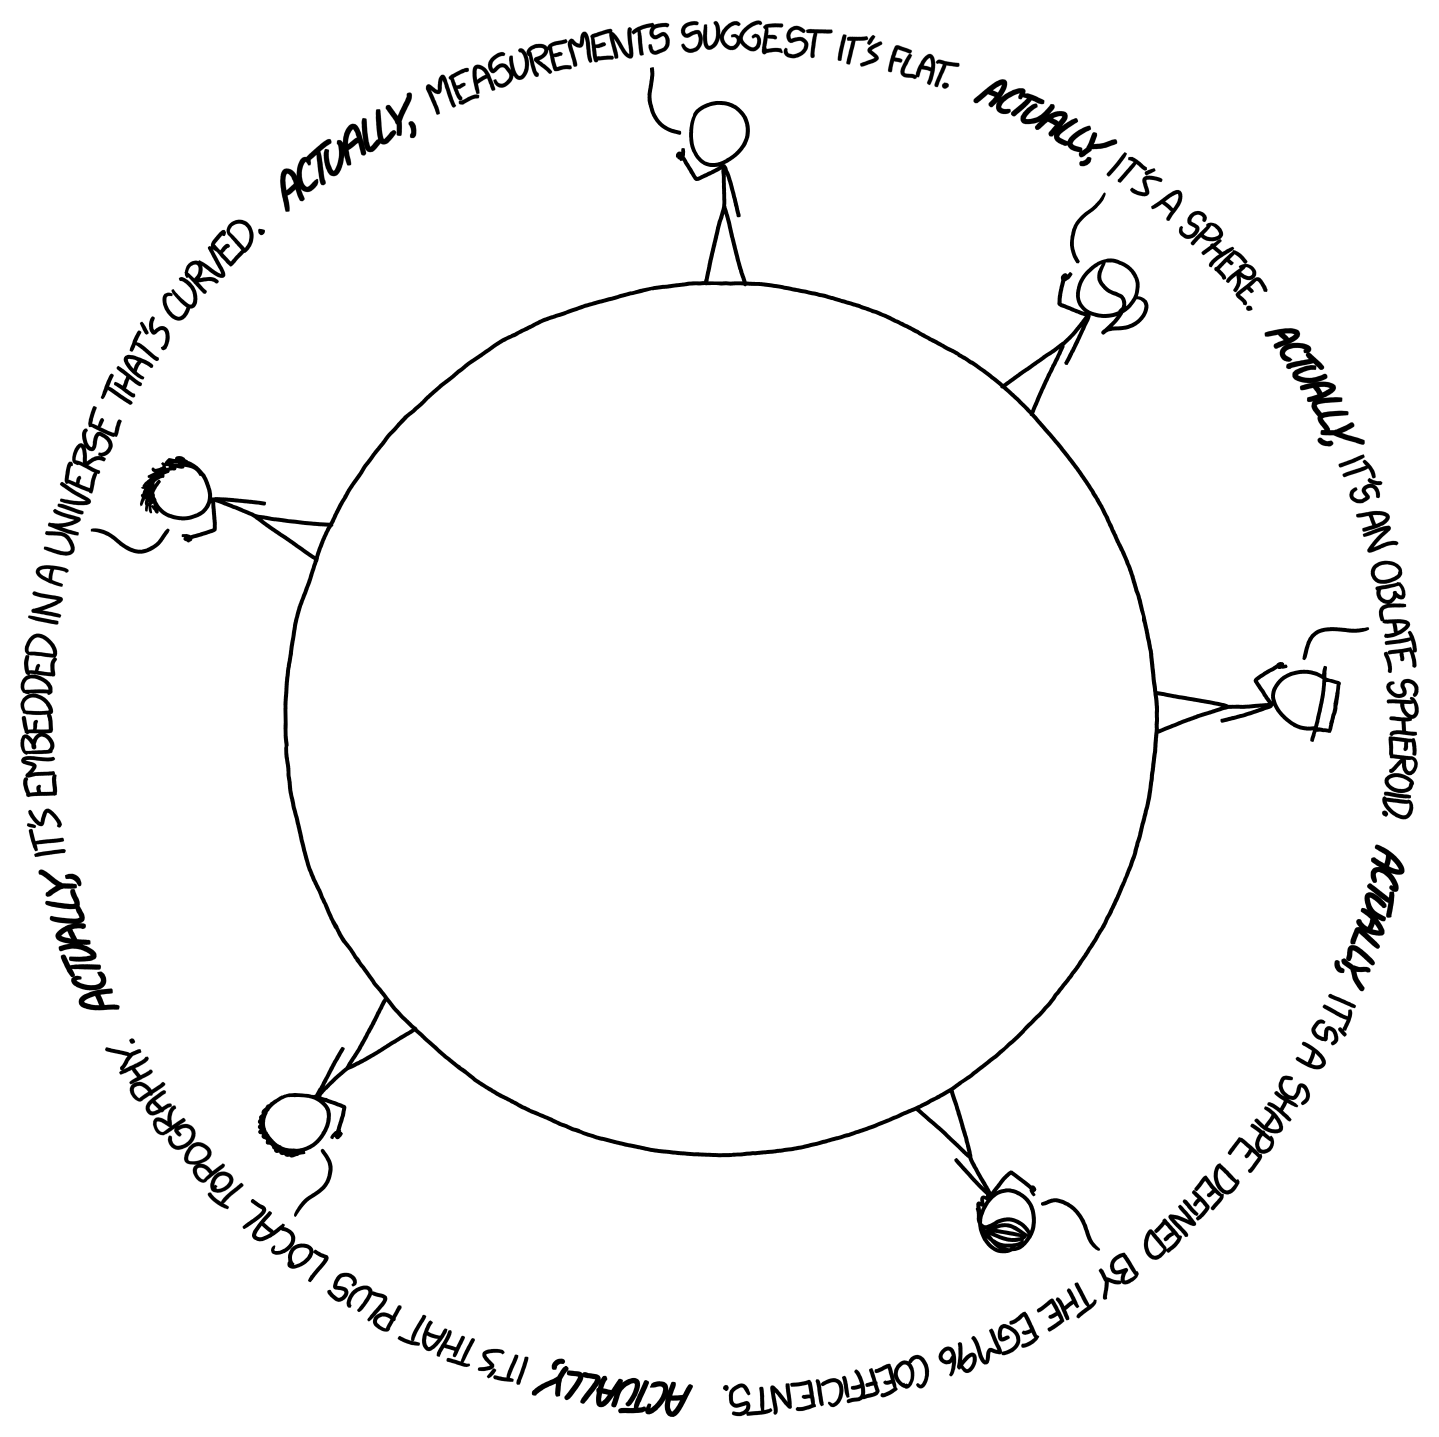
\includegraphics{images/actually_2x.png}
\end{center}

\setlength{\abovedisplayskip}{-5pt}
\setlength{\abovedisplayshortskip}{-5pt}

{
\hypersetup{linkcolor=}
\setcounter{tocdepth}{2}
\tableofcontents
}
\listoffigures
\listoftables
\hypertarget{prefazione}{%
\chapter*{Prefazione}\label{prefazione}}


La presente dispensa contiene il materiale delle lezioni dell'insegnamento di \emph{Costruzione e validazione di strumenti di misura dell'efficacia dell'intervento psicologico in neuropsicologia} B020881 (B213) rivolto agli studenti del secondo anno del Corso di Laurea Magistrale in Psicologia Clinica e della Salute e Neuropsicologia (curriculum: assessment e intervento psicologici in neuropsicologia - E21), A.A. 2021-2022. L'insegnamento si propone di fornire agli studenti un'introduzione all'assessment psicologico, ovvero un insieme di conoscenze/competenze che si pongono all'intersezione tra psicometria, statistica e informatica.

Nello specifico, l'insegnamento si focalizzerà sull'analisi fattoriale confermativa (\emph{confermatory factor analysis}, CFA) e sull'analisi fattoriale esplorativa, (\emph{explorative factor analysis}, EFA), cioè sugli strumenti che vengono usati durante il processo di sviluppo dei test psicometrici, ovvero che vengono usati per esaminare la struttura latente di una scala psicologica (ad esempio un questionario). In questo contesto, la CFA viene utilizzata per verificare il numero di dimensioni sottostanti gli indicatori (fattori) e l'intensità delle relazioni item-fattore (saturazioni fattoriali). La CFA consente anche di capire di come dovrebbe essere svolto lo scoring di un test. Quando la struttura latente è multifattoriale (cioè, a due o più fattori), il numero di fattori è indicativo del numero di sottoscale e di come esse dovrebbero essere codificate. La CFA è un importante strumento analitico anche per altri aspetti della valutazione psicometrica. Può essere utilizzata per stimare l'affidabilità di scala dei test psicometrici in modo da evitare i problemi della teoria classica dei test (ad es. alpha di Cronbach). Dati i recenti progressi nell'analisi dei dati categoriali, ora la CFA offre un quadro analitico comparabile a quello offerto dalla teoria di risposta agli item (IRT). In effetti, secondo \citet{brown2015confirmatory}, la CFA offre una maggiore flessibilità analitica rispetto al modello IRT tradizionale.

Un costrutto è un concetto teorico che può essere operazionalizzato nei termini di un fattore. In psicologia clinica, psichiatria e neuropsicologia, ad esempio, i disturbi mentali sono costrutti manifestati da vari insiemi di sintomi che sono riportati dal paziente o osservati da altri. La CFA è uno strumento analitico indispensabile per la validazione dei costrutti psicologici. I risultati della CFA possono fornire prove convincenti della validità convergente e discriminante dei costrutti teorici. La validità convergente è indicata dall'evidenza che diversi indicatori di costrutti teoricamente simili o sovrapposti sono fortemente correlati. La validità discriminante è indicata dai risultati che mostrano che gli indicatori di costrutti teoricamente distinti sono altamente incorrelati. Un punto di forza fondamentale degli approcci CFA per la costruzione e la validazione di uno strumento psicometrico è che le risultanti stime di validità convergente e discriminante sono corrette per l'errore di misurazione. Pertanto, la CFA fornisce un quadro analitico migliore rispetto ai metodi tradizionali che non tengono conto dell'errore di misurazione (ad esempio, gli approcci ordinari ai minimi quadrati come la correlazione/regressione multipla, i quali presuppongono che le variabili nell'analisi siano prive di errori di misurazione).

Spesso, parte della covariazione delle misure osservate è dovuta a fonti diverse dai fattori latenti di interesse. Questa covariazione aggiuntiva spesso riflette la varianza del metodo utilizzato per la misurazione. Gli effetti del metodo possono verificarsi anche all'interno di un'unica modalità di valutazione. Ad esempio, effetti del metodo sono solitamente presenti nei questionari che contengono una combinazione di elementi formulati positivamente e negativamente. Sfortunatamente, l'EFA non è in grado di stimare gli effetti del metodo. In effetti, l'uso di EFA quando esistono effetti del metodo può produrre risultati fuorvianti, ovvero suggerire la presenza di fattori aggiuntivi che corrispondono invece ad artefatti della misurazione. Nella CFA, invece, gli effetti del metodo possono essere specificati come parte della teoria dell'errore del modello di misurazione.

Un altro punto di forza della CFA è la sua capacità di affrontare il problema della generalizzabilità del modello di misurazione tra gruppi di individui o nel tempo. La valutazione dell'invarianza della misura è un aspetto importante dello sviluppo del test. Se un test è destinato a essere somministrato in una popolazione eterogenea, si dovrebbe stabilire che le sue proprietà di misurazione sono equivalenti in sottogruppi della popolazione (es. sesso, razza). Si dice che un test è distorto quando alcuni dei suoi elementi non misurano il costrutto sottostante in modo comparabile tra gruppi di rispondenti. Il test fornisce una stima distorta se, ad esempio, per un dato livello di vera intelligenza, gli uomini tendono a ottenere un punteggio di QI più alto rispetto alle donne. Il problema della generalizzabilità della validità del costrutto tra i gruppi può essere affrontato nella CFA esaminando gruppi multipli mediante modelli MIMIC (indicatori multipli, cause multiple). Inotre, è possibile chiedersi se il modello di misurazione sia equivalente tra i gruppi. Le soluzioni CFA a gruppi multipli vengono anche utilizzate per esaminare l'invarianza della misurazione longitudinale. Questo è un aspetto molto importante dell'analisi delle variabili latenti dei progetti di misure ripetute. In assenza di tale valutazione, non è possibile determinare se il cambiamento temporale in un costrutto sia dovuto a un vero cambiamento dei rispondenti o a cambiamenti nel modo di rispondere alla scala nel tempo. L'analisi a gruppi multipli può essere applicata a qualsiasi tipo di modello CFA. Ad esempio, queste procedure possono essere incorporate nell'analisi dei dati multitratto-multimetodo per esaminare la generalizzabilità della validità del costrutto tra gruppi.

In questo insegnamento la discussione delle teciche della CFA sarà preceduta da un'introduzione relativa alla EFA e la teoria classica dei test. La EFA, infatti, può essere concepita il metodo che viene utilizzato nei primi passi dello sviluppo di una scala psicometria, mentre la teoria classica dei test rappresenta la cornice teorica di partenza, di cui la CFA e i modelli di equazioni strutturali costituiscono uno sviluppo.

L'insegnamento pone una grande enfasi non solo sulla comprensione dei concetti teorici necessari per la costruzione e la validazione di uno strumento di misura in psicologia, ma anche sulla capacità di applicare tali concetti in situazioni concrete. Di conseguenza, la discussione dei concetti sarà sempre accompagnata da applicazioni pratiche. Tali applicazioni richiedono l'uso di un software. In questo insegnamento useremo \(\textsf{R}\) \citep{rmanual} quale linguaggio di programmazione probabilistica e, tra gli altri, il pacchetto \texttt{lavaan} che consente di svolgere le analisi statistiche della CFA e della EFA \citep{beaujean2014latent}. La teoria classica dei test verrà descritta con riferimento al classico testo di \citet{lord1968statistical}. Questa dispensa, inoltre, segue da vicino la trattazione della CFA fornita nei testi di \citet{mcdonald2013test} e di \citet{brown2015confirmatory}.

Trattando di argomenti avanzati, questo insegnamento presuppone la conoscenza di base dei concetti fondamentali della teoria delle probabilità; presuppone inoltre il possesso delle conoscenze di base necessarie per procedere all'utilizzo di \(\textsf{R}\). Informazioni su tali argomenti sono forniti nella dispensa di Psicometria (A.A. 2021-2022).

\begin{flushright}
Corrado Caudek\\
Marzo 2022 \end{flushright}

\mainmatter

\hypertarget{part-il-modello-lineare}{%
\part{Il modello lineare}\label{part-il-modello-lineare}}

\hypertarget{lanalisi-di-regressione}{%
\chapter{L'analisi di regressione}\label{lanalisi-di-regressione}}

Conoscere l'analisi di regressione aiuta a capire la teoria classica dei test, l'analisi fattoriale e i modelli di equazioni strutturali. Sebbene le tecniche dell'analisi di regressione analizzino solo le variabili osservate, i principi della regressione costituiscono la base delle tecniche più avanzate che includono anche le variabili latenti.

\hypertarget{regressione-bivariata}{%
\section{Regressione bivariata}\label{regressione-bivariata}}

Il modello di regressione bivariata descrive l'associazione tra il valore atteso di \(Y \mid x_i\) e \(x\) nei termini di una relazione lineare:

\[
\mathbb{E}(Y \mid x_i) = \alpha + \beta x_i,
\] dove i valori \(x_i\) sono considerati fissi per disegno. Nel modello ``classico'', si assume che le distribuzioni \(Y \mid x_i\) siano Normali con deviazione standard \(\sigma_\varepsilon\).

Il significato dei coefficienti di regressione è semplice:

\begin{itemize}
\tightlist
\item
  \(\alpha\) è il valore atteso di \(Y\) quando \(X = 0\);
\item
  \(\beta\) è l'incremento atteso nel valore atteso di \(Y\) quando \(X\) aumenta di un'unità.
\end{itemize}

Per fare un esempio, consideriamo i dati dell'antropologo Sahlins, il quale si è chiesto se esiste un'associazione tra l'ampiezza del clan (\texttt{consumers}) e l'area occupata da quel clan (\texttt{acres}) in una popolazione di cacciatori-raccoglitori. I dati sono i seguenti:

\begin{Shaded}
\begin{Highlighting}[]
\FunctionTok{data}\NormalTok{(Sahlins)}
\FunctionTok{head}\NormalTok{(Sahlins)}
\CommentTok{\#\textgreater{}   consumers acres}
\CommentTok{\#\textgreater{} 1      1.00  1.71}
\CommentTok{\#\textgreater{} 2      1.08  1.52}
\CommentTok{\#\textgreater{} 3      1.15  1.29}
\CommentTok{\#\textgreater{} 4      1.15  3.09}
\CommentTok{\#\textgreater{} 5      1.20  2.21}
\CommentTok{\#\textgreater{} 6      1.30  2.26}
\end{Highlighting}
\end{Shaded}

\begin{Shaded}
\begin{Highlighting}[]
\NormalTok{Sahlins }\SpecialCharTok{\%\textgreater{}\%}
  \FunctionTok{ggplot}\NormalTok{(}\FunctionTok{aes}\NormalTok{(}\AttributeTok{x =}\NormalTok{ consumers, }\AttributeTok{y =}\NormalTok{ acres)) }\SpecialCharTok{+}
  \FunctionTok{geom\_point}\NormalTok{() }\SpecialCharTok{+}
  \FunctionTok{geom\_smooth}\NormalTok{(}\AttributeTok{method =}\NormalTok{ lm, }\AttributeTok{se =} \ConstantTok{FALSE}\NormalTok{)}
\end{Highlighting}
\end{Shaded}

\begin{center}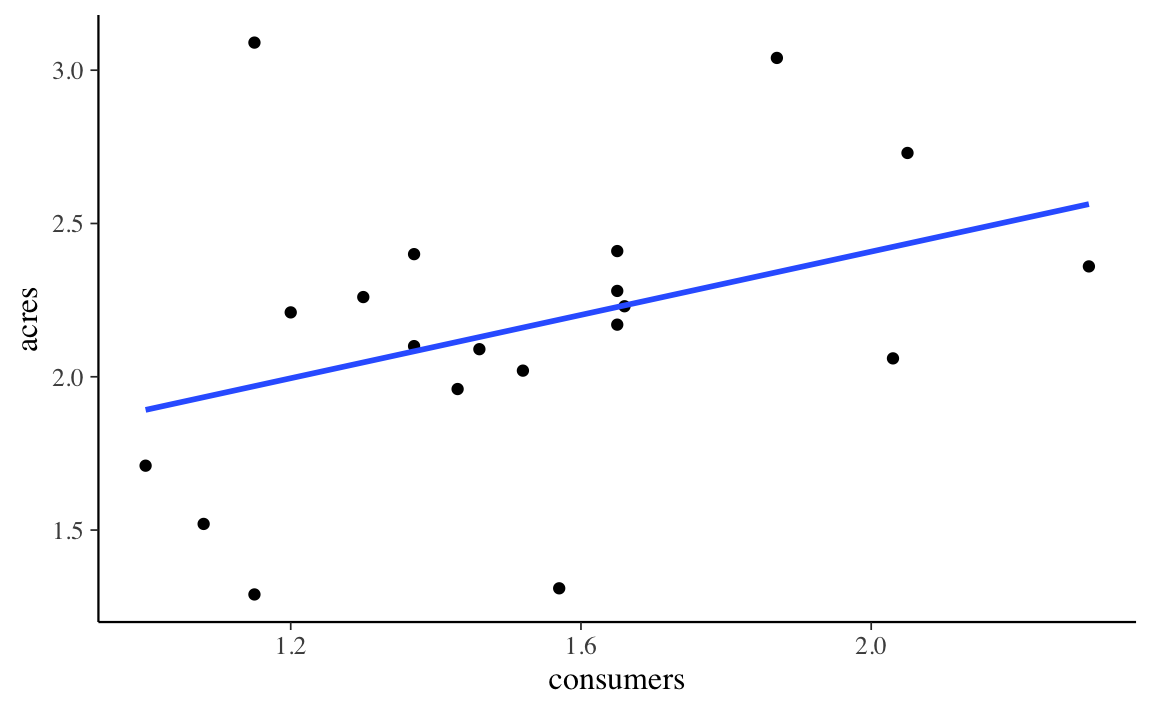
\includegraphics{cfa_book_files/figure-latex/unnamed-chunk-4-1} \end{center}

\begin{Shaded}
\begin{Highlighting}[]
\NormalTok{fm }\OtherTok{\textless{}{-}} \FunctionTok{lm}\NormalTok{(acres }\SpecialCharTok{\textasciitilde{}}\NormalTok{ consumers, }\AttributeTok{data =}\NormalTok{ Sahlins)}
\NormalTok{fm}\SpecialCharTok{$}\NormalTok{coef}
\CommentTok{\#\textgreater{} (Intercept)   consumers }
\CommentTok{\#\textgreater{}      1.3756      0.5163}
\end{Highlighting}
\end{Shaded}

Dalla figura notiamo che, se \texttt{consumers} aumenta di un'unità (da 1.2 a 2.2), allora la retta di regressione (ovvero, il valore atteso di \(Y\)) aumenta di circa 0.5 punti -- esattamente, aumenta di 0.5163 punti, come indicato dalla stima del coefficiente \(\beta\). L'interpretazione del coefficiente \(\alpha\) è più problematica, perché non ha senso pensare ad un clan di ampiezza 0. Per affrontare questo problema, centriamo il predittore.

\hypertarget{regressori-centrati}{%
\subsection{Regressori centrati}\label{regressori-centrati}}

Esprimiamo la variabile \texttt{consumers} nei termini degli scarti dalla media:

\begin{Shaded}
\begin{Highlighting}[]
\NormalTok{Sahlins }\OtherTok{\textless{}{-}}\NormalTok{ Sahlins }\SpecialCharTok{\%\textgreater{}\%}
  \FunctionTok{mutate}\NormalTok{(}
    \AttributeTok{xc =}\NormalTok{ consumers }\SpecialCharTok{{-}} \FunctionTok{mean}\NormalTok{(consumers)}
\NormalTok{  )}
\end{Highlighting}
\end{Shaded}

Svolgiamo nuovamente l'analisi di regressione con il nuovo predittore:

\begin{Shaded}
\begin{Highlighting}[]
\NormalTok{fm1 }\OtherTok{\textless{}{-}} \FunctionTok{lm}\NormalTok{(acres }\SpecialCharTok{\textasciitilde{}}\NormalTok{ xc, }\AttributeTok{data =}\NormalTok{ Sahlins)}
\NormalTok{fm1}\SpecialCharTok{$}\NormalTok{coef}
\CommentTok{\#\textgreater{} (Intercept)          xc }
\CommentTok{\#\textgreater{}      2.1620      0.5163}
\end{Highlighting}
\end{Shaded}

\begin{Shaded}
\begin{Highlighting}[]
\NormalTok{Sahlins }\SpecialCharTok{\%\textgreater{}\%}
  \FunctionTok{ggplot}\NormalTok{(}\FunctionTok{aes}\NormalTok{(}\AttributeTok{x =}\NormalTok{ xc, }\AttributeTok{y =}\NormalTok{ acres)) }\SpecialCharTok{+}
  \FunctionTok{geom\_point}\NormalTok{() }\SpecialCharTok{+}
  \FunctionTok{geom\_smooth}\NormalTok{(}\AttributeTok{method =}\NormalTok{ lm, }\AttributeTok{se =} \ConstantTok{FALSE}\NormalTok{)}
\end{Highlighting}
\end{Shaded}

\begin{center}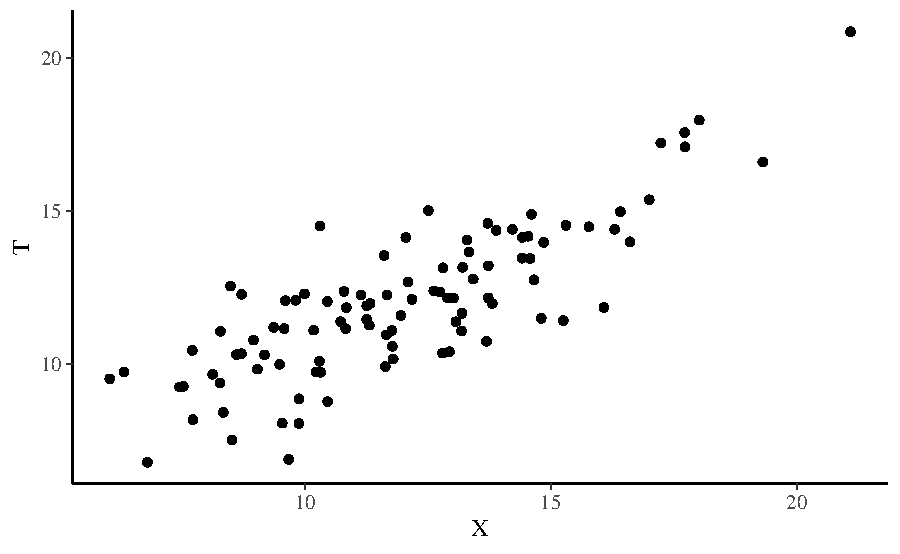
\includegraphics{cfa_book_files/figure-latex/unnamed-chunk-8-1} \end{center}

La stima di \(\beta\) è rimasta invariata ma ora possiamo attribuire un significato alla stima di \(\alpha\): questo coefficiente indica il valore atteso della \(Y\) quando \(X\) assume il suo valore medio.

\hypertarget{minimi-quadrati}{%
\subsection{Minimi quadrati}\label{minimi-quadrati}}

La stima dei coefficienti del modello di regressione può essere effettuata in modi diversi: massima verosimiglianza o metodi bayesiani. Se ci limitiamo qui alla massima verosimiglianza possiamo semplificare il problema assumento che le distribuzioni condizionate \(Y \mid x\) siano Normali. In tali circostanze, la stima dei coefficienti del modello di regressione può essere trovata con il metodo dei minimi quadrati.

In pratica, questo significa trovare i coefficienti \(a\) e \(b\) che minimizzano

\[
SS_{\text{res}} = \sum(y_i - \hat{y}_i)^2,
\] con \(\hat{y}_i = a + b x_i\).

Per fornire un'idea di come questo viene fatto, usiamo una simulazione. Per semplicità, supponiamo di conoscere \(a = 1.3756445\) e di volere stimare \(b\).

\begin{Shaded}
\begin{Highlighting}[]
\NormalTok{x }\OtherTok{\textless{}{-}}\NormalTok{ Sahlins}\SpecialCharTok{$}\NormalTok{consumers}
\NormalTok{y }\OtherTok{\textless{}{-}}\NormalTok{ Sahlins}\SpecialCharTok{$}\NormalTok{acres}
\NormalTok{a }\OtherTok{\textless{}{-}} \FloatTok{1.3756445}

\NormalTok{nrep }\OtherTok{\textless{}{-}} \FloatTok{1e3}
\NormalTok{b }\OtherTok{\textless{}{-}} \FunctionTok{seq}\NormalTok{(}\DecValTok{0}\NormalTok{, }\DecValTok{1}\NormalTok{, }\AttributeTok{length.out =}\NormalTok{ nrep)}

\NormalTok{ssres }\OtherTok{\textless{}{-}} \FunctionTok{rep}\NormalTok{(}\ConstantTok{NA}\NormalTok{, nrep)}
\ControlFlowTok{for}\NormalTok{ (i }\ControlFlowTok{in} \DecValTok{1}\SpecialCharTok{:}\NormalTok{nrep) \{}
\NormalTok{  yhat }\OtherTok{\textless{}{-}}\NormalTok{ a }\SpecialCharTok{+}\NormalTok{ b[i] }\SpecialCharTok{*}\NormalTok{ x}
\NormalTok{  ssres[i] }\OtherTok{\textless{}{-}} \FunctionTok{sum}\NormalTok{((y }\SpecialCharTok{{-}}\NormalTok{ yhat)}\SpecialCharTok{\^{}}\DecValTok{2}\NormalTok{)}
\NormalTok{\}}
\end{Highlighting}
\end{Shaded}

Un grafico di \(SS_{\text{res}}\) in funzione di \(b\) mostra che il valore \(b\) che minimizza \(SS_{\text{res}}\) corrisponde, appunto, a 0.5163.

\begin{Shaded}
\begin{Highlighting}[]
\FunctionTok{tibble}\NormalTok{(b, ssres) }\SpecialCharTok{\%\textgreater{}\%}
  \FunctionTok{ggplot}\NormalTok{(}\FunctionTok{aes}\NormalTok{(}\AttributeTok{x =}\NormalTok{ b, }\AttributeTok{y =}\NormalTok{ ssres)) }\SpecialCharTok{+}
  \FunctionTok{geom\_line}\NormalTok{()}
\end{Highlighting}
\end{Shaded}

\begin{center}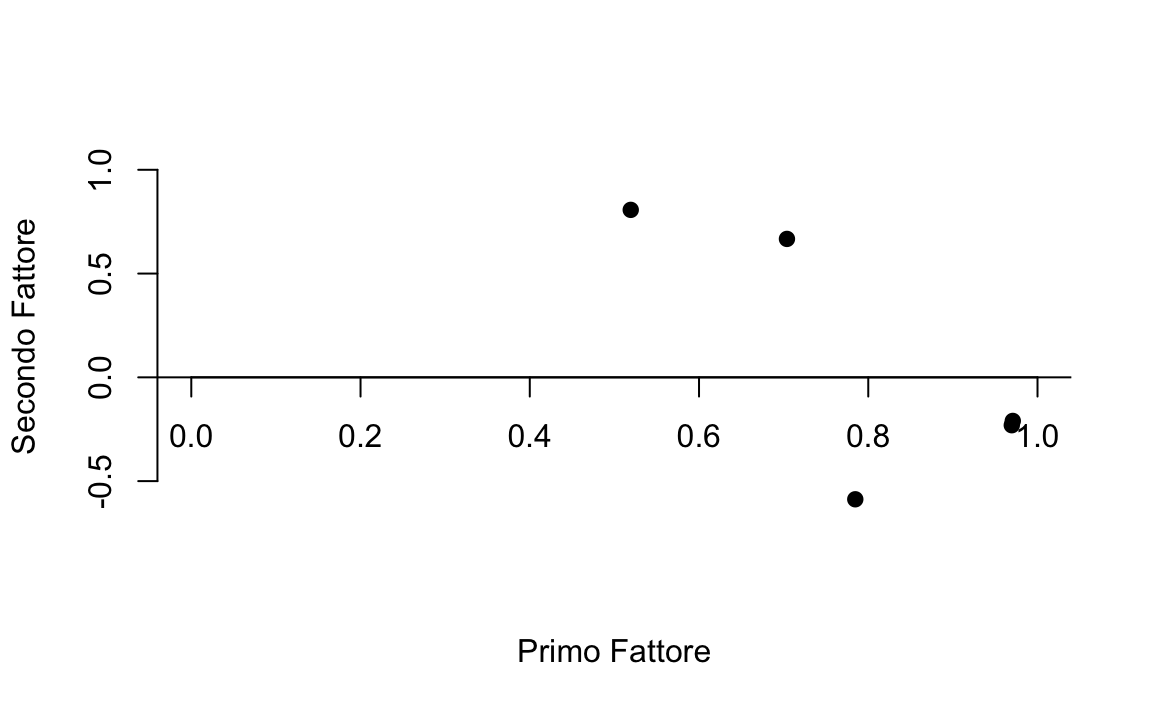
\includegraphics{cfa_book_files/figure-latex/unnamed-chunk-10-1} \end{center}

\hypertarget{relazione-tra-b-e-r}{%
\subsection{\texorpdfstring{Relazione tra \(b\) e \(r\)}{Relazione tra b e r}}\label{relazione-tra-b-e-r}}

Un altro modo per interpretare \(b\) è quello di considerare la relazione tra la pendenza della retta di regressione e il coefficiente di correlazione:

\[
b_X = r_{XY} \frac{S_X}{S_Y}
\]

L'equazione precedente rende chiaro che, se i dati sono standardizzati, \(b = r\).

Verifichiamo:

\begin{Shaded}
\begin{Highlighting}[]
\NormalTok{Sahlins }\SpecialCharTok{\%\textgreater{}\%}
\NormalTok{  dplyr}\SpecialCharTok{::}\FunctionTok{select}\NormalTok{(acres, consumers) }\SpecialCharTok{\%\textgreater{}\%}
  \FunctionTok{cor}\NormalTok{()}
\CommentTok{\#\textgreater{}            acres consumers}
\CommentTok{\#\textgreater{} acres     1.0000    0.3757}
\CommentTok{\#\textgreater{} consumers 0.3757    1.0000}
\end{Highlighting}
\end{Shaded}

\begin{Shaded}
\begin{Highlighting}[]
\NormalTok{fm2 }\OtherTok{\textless{}{-}} \FunctionTok{lm}\NormalTok{(}\FunctionTok{scale}\NormalTok{(acres) }\SpecialCharTok{\textasciitilde{}} \FunctionTok{scale}\NormalTok{(consumers), }\AttributeTok{data =}\NormalTok{ Sahlins)}
\NormalTok{fm2}\SpecialCharTok{$}\NormalTok{coef}
\CommentTok{\#\textgreater{}      (Intercept) scale(consumers) }
\CommentTok{\#\textgreater{}        9.917e{-}17        3.757e{-}01}
\end{Highlighting}
\end{Shaded}

\hypertarget{attenuazione}{%
\subsection{Attenuazione}\label{attenuazione}}

Il fenomeno dell'attenuazione si verifica quando \(X\) viene misurato con una componente di errore. Esaminiamo la seguente simulazione.

\begin{Shaded}
\begin{Highlighting}[]
\FunctionTok{set.seed}\NormalTok{(}\DecValTok{1234}\NormalTok{)}
\NormalTok{n }\OtherTok{\textless{}{-}} \DecValTok{100}
\NormalTok{x }\OtherTok{\textless{}{-}} \FunctionTok{rnorm}\NormalTok{(n, }\DecValTok{10}\NormalTok{, }\FloatTok{1.5}\NormalTok{)}
\NormalTok{y }\OtherTok{\textless{}{-}} \FloatTok{1.5} \SpecialCharTok{*}\NormalTok{ x }\SpecialCharTok{+} \FunctionTok{rnorm}\NormalTok{(n, }\DecValTok{0}\NormalTok{, }\DecValTok{2}\NormalTok{)}
\FunctionTok{tibble}\NormalTok{(x, y) }\SpecialCharTok{\%\textgreater{}\%}
  \FunctionTok{ggplot}\NormalTok{(}\FunctionTok{aes}\NormalTok{(x, y)) }\SpecialCharTok{+}
  \FunctionTok{geom\_point}\NormalTok{()}
\end{Highlighting}
\end{Shaded}

\begin{center}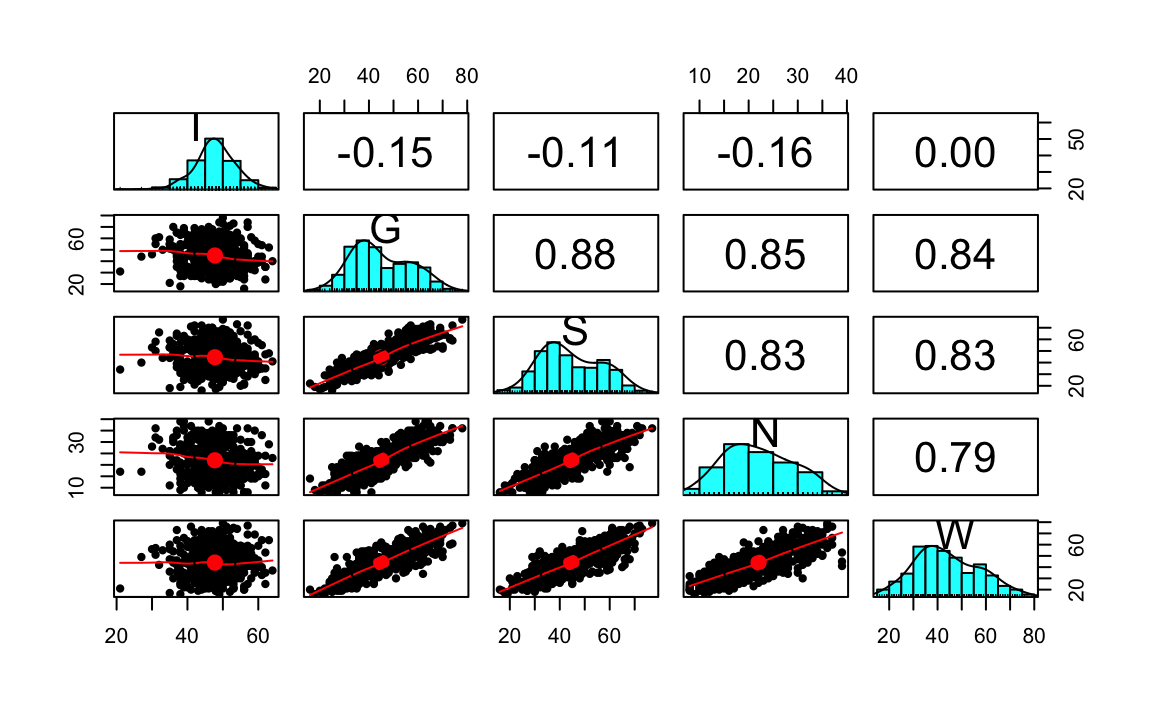
\includegraphics{cfa_book_files/figure-latex/unnamed-chunk-13-1} \end{center}

\begin{Shaded}
\begin{Highlighting}[]
\NormalTok{sim\_dat }\OtherTok{\textless{}{-}} \FunctionTok{tibble}\NormalTok{(x, y)}
\NormalTok{fm }\OtherTok{\textless{}{-}} \FunctionTok{lm}\NormalTok{(y }\SpecialCharTok{\textasciitilde{}}\NormalTok{ x, sim\_dat)}
\NormalTok{fm}\SpecialCharTok{$}\NormalTok{coef}
\CommentTok{\#\textgreater{} (Intercept)           x }
\CommentTok{\#\textgreater{}      0.4221      1.4652}
\end{Highlighting}
\end{Shaded}

Questi sono i coefficienti di regressione quando \(X\) è misurata senza errori.

\begin{Shaded}
\begin{Highlighting}[]
\NormalTok{sim\_dat }\OtherTok{\textless{}{-}}\NormalTok{ sim\_dat }\SpecialCharTok{\%\textgreater{}\%}
  \FunctionTok{mutate}\NormalTok{(}
    \AttributeTok{x1 =}\NormalTok{ x }\SpecialCharTok{+} \FunctionTok{rnorm}\NormalTok{(n, }\DecValTok{0}\NormalTok{, }\DecValTok{2}\NormalTok{)}
\NormalTok{  )}

\NormalTok{fm1 }\OtherTok{\textless{}{-}} \FunctionTok{lm}\NormalTok{(y }\SpecialCharTok{\textasciitilde{}}\NormalTok{ x1, sim\_dat)}
\NormalTok{fm1}\SpecialCharTok{$}\NormalTok{coef}
\CommentTok{\#\textgreater{} (Intercept)          x1 }
\CommentTok{\#\textgreater{}      8.3872      0.6296}
\end{Highlighting}
\end{Shaded}

Aggiungendo una componente d'errore su \(X\), la grandezza del coefficiente \(b\) diminuisce.

\hypertarget{coefficiente-di-determinazione}{%
\subsection{Coefficiente di determinazione}\label{coefficiente-di-determinazione}}

Tecnicamente, il coefficiente di determinazione è dato da:

\[
R^2 = \frac{\sum(\hat{y} - \bar{y})^2}{\sum(y_i - \bar{y})^2}
\]

Al denominatore abbiamo la \emph{devianza totale}, ovvero una misura della dispersione di \(y_i\) rispetto alla media \(\bar{y}\). Al numeratore abbiamo una misura della dispersione del valore atteso della \(Y\) rispetto alla sua media. Il rapporto, dunque, ci dice qual è la quota della variabilità totale di \(Y\) che può essere predetta in base al modello lineare.

Per i dati di Sahlins abbiamo:

\begin{Shaded}
\begin{Highlighting}[]
\NormalTok{mod }\OtherTok{\textless{}{-}} \FunctionTok{lm}\NormalTok{(acres }\SpecialCharTok{\textasciitilde{}}\NormalTok{ consumers, }\AttributeTok{data =}\NormalTok{ Sahlins)}
\NormalTok{a }\OtherTok{\textless{}{-}}\NormalTok{ mod}\SpecialCharTok{$}\NormalTok{coef[}\DecValTok{1}\NormalTok{]}
\NormalTok{b }\OtherTok{\textless{}{-}}\NormalTok{ mod}\SpecialCharTok{$}\NormalTok{coef[}\DecValTok{2}\NormalTok{]}
\NormalTok{yhat }\OtherTok{\textless{}{-}}\NormalTok{ a }\SpecialCharTok{+}\NormalTok{ b }\SpecialCharTok{*}\NormalTok{ Sahlins}\SpecialCharTok{$}\NormalTok{consumers}
\NormalTok{ss\_tot }\OtherTok{\textless{}{-}} \FunctionTok{sum}\NormalTok{((Sahlins}\SpecialCharTok{$}\NormalTok{acres }\SpecialCharTok{{-}} \FunctionTok{mean}\NormalTok{(Sahlins}\SpecialCharTok{$}\NormalTok{acres))}\SpecialCharTok{\^{}}\DecValTok{2}\NormalTok{)}
\NormalTok{ss\_reg }\OtherTok{\textless{}{-}} \FunctionTok{sum}\NormalTok{((yhat }\SpecialCharTok{{-}} \FunctionTok{mean}\NormalTok{(Sahlins}\SpecialCharTok{$}\NormalTok{acres))}\SpecialCharTok{\^{}}\DecValTok{2}\NormalTok{)}
\NormalTok{r2 }\OtherTok{\textless{}{-}}\NormalTok{ ss\_reg }\SpecialCharTok{/}\NormalTok{ ss\_tot}
\NormalTok{r2}
\CommentTok{\#\textgreater{} [1] 0.1411}
\end{Highlighting}
\end{Shaded}

Verifichiamo:

\begin{Shaded}
\begin{Highlighting}[]
\FunctionTok{summary}\NormalTok{(mod)}
\CommentTok{\#\textgreater{} }
\CommentTok{\#\textgreater{} Call:}
\CommentTok{\#\textgreater{} lm(formula = acres \textasciitilde{} consumers, data = Sahlins)}
\CommentTok{\#\textgreater{} }
\CommentTok{\#\textgreater{} Residuals:}
\CommentTok{\#\textgreater{}     Min      1Q  Median      3Q     Max }
\CommentTok{\#\textgreater{} {-}0.8763 {-}0.1873 {-}0.0211  0.2135  1.1206 }
\CommentTok{\#\textgreater{} }
\CommentTok{\#\textgreater{} Coefficients:}
\CommentTok{\#\textgreater{}             Estimate Std. Error t value Pr(\textgreater{}|t|)   }
\CommentTok{\#\textgreater{} (Intercept)    1.376      0.468    2.94   0.0088 **}
\CommentTok{\#\textgreater{} consumers      0.516      0.300    1.72   0.1026   }
\CommentTok{\#\textgreater{} {-}{-}{-}}
\CommentTok{\#\textgreater{} Signif. codes:  }
\CommentTok{\#\textgreater{} 0 \textquotesingle{}***\textquotesingle{} 0.001 \textquotesingle{}**\textquotesingle{} 0.01 \textquotesingle{}*\textquotesingle{} 0.05 \textquotesingle{}.\textquotesingle{} 0.1 \textquotesingle{} \textquotesingle{} 1}
\CommentTok{\#\textgreater{} }
\CommentTok{\#\textgreater{} Residual standard error: 0.454 on 18 degrees of freedom}
\CommentTok{\#\textgreater{} Multiple R{-}squared:  0.141,  Adjusted R{-}squared:  0.0934 }
\CommentTok{\#\textgreater{} F{-}statistic: 2.96 on 1 and 18 DF,  p{-}value: 0.103}
\end{Highlighting}
\end{Shaded}

Da cui deriva che \(R^2\) è uguale al quadrato del coefficiente di correlazione:

\begin{Shaded}
\begin{Highlighting}[]
\FunctionTok{cor}\NormalTok{(Sahlins}\SpecialCharTok{$}\NormalTok{acres, Sahlins}\SpecialCharTok{$}\NormalTok{consumers)}\SpecialCharTok{\^{}}\DecValTok{2}
\CommentTok{\#\textgreater{} [1] 0.1411}
\end{Highlighting}
\end{Shaded}

\hypertarget{errore-standard-della-regressione}{%
\subsection{Errore standard della regressione}\label{errore-standard-della-regressione}}

L'errore standard della regressione è una stima della dispersione di \(y \mid x_i\) nella popolazione. Non è altro che la deviazione standard dei residui

\[
e = y_i - \hat{y}_i
\]

che, al denominatore, riporta \(n-2\). La ragione è che, per calcolare \(\hat{y}\), vengono ``perduti'' due gradi di libertà -- il calcolo di \(\hat{y}\) è basato sulla stima di due coefficienti: \(a\) e \(b\).

\begin{Shaded}
\begin{Highlighting}[]
\NormalTok{e }\OtherTok{\textless{}{-}}\NormalTok{ yhat }\SpecialCharTok{{-}}\NormalTok{ Sahlins}\SpecialCharTok{$}\NormalTok{acres}
\NormalTok{(}\FunctionTok{sum}\NormalTok{(e}\SpecialCharTok{\^{}}\DecValTok{2}\NormalTok{) }\SpecialCharTok{/}\NormalTok{ (}\FunctionTok{length}\NormalTok{(Sahlins}\SpecialCharTok{$}\NormalTok{acres) }\SpecialCharTok{{-}} \DecValTok{2}\NormalTok{)) }\SpecialCharTok{\%\textgreater{}\%}
  \FunctionTok{sqrt}\NormalTok{()}
\CommentTok{\#\textgreater{} [1] 0.4543}
\end{Highlighting}
\end{Shaded}

Il valore trovato corrisponde a quello riportato nell'output di \texttt{lm()}.

\hypertarget{regressione-multipla}{%
\section{Regressione multipla}\label{regressione-multipla}}

Nella regressione multipla vengono utilizzati \(k > 1\) predittori:

\[
y_i = \alpha + \sum_{j=1}^k \beta_j x_i + \varepsilon_i.
\] L'interpretazione geometrica è simile a quella del modello bivariato. Nel caso di due predittori, il valore atteso della \(y\) può essere rappresentato da un piano; nel caso di \(k > 2\) predittori, da un iper-piano. Nel caso di \(k=2\), tale piano è posto in uno spazio di dimensioni \(x_1\), \(x_2\) (che possiamo immaginare definire un piano orizzontale) e \(y\) (ortogonale a tale piano). La superficie piana che rappresenta \(\mathbb{E}(y)\) è inclinata in maniera tale che l'angolo tra il piano e l'asse \(x_1\) corrisponde a \(\beta_1\) e l'angolo tra il piano e l'asse \(x_2\) corrisponde a \(\beta_2\).

\hypertarget{significato-dei-coefficienti-parziali-di-regressione}{%
\subsection{Significato dei coefficienti parziali di regressione}\label{significato-dei-coefficienti-parziali-di-regressione}}

Ai coefficienti parziali del modello di regressione multipla possiamo assegnare la seguente interpretazione:

\emph{Il coefficiente parziale di regressione \(\beta_j\) rappresenta l'incremento atteso della \(y\) se \(x_j\) viene incrementata di un'unità, tenendo costante il valore delle altre variabili indipendenti.}

Un modo per interpretare la locuzione ``al netto dell'effetto delle altre variabili indipendenti'' è quello di esaminare la relazione tra la \(y\) parzializzata e la \(x_j\) parzializzata. In questo contesto, parzializzare significa decomporre una variabile di due componenti: una componente che è linearmente predicibile da una o più altre variabili e una componente che è linearmente incorrelata con tali varibili ``terze''.

Eseguiamo questa ``depurazione'' dell'effetto delle variabili ``terze'' sia sulla \(y\) sia su \(x_j\). A questo punto possiamo esaminare la relazione bivariata che intercorre tra la componente della \(y\) linearmente indipendente dalle variabili ``terze'' e la componente della \(x_j\) linearmente indipendente dalle variabili ``terze''. Il coefficiente di regressione bivariato così ottenuto è identico al coefficiente parziale di regressione nel modello di regressione multipla. Possiamo così ottenere un'interpretazione di \(\beta_j\).

Esaminiamo un caso concreto.

\begin{Shaded}
\begin{Highlighting}[]
\NormalTok{d }\OtherTok{\textless{}{-}}\NormalTok{ rio}\SpecialCharTok{::}\FunctionTok{import}\NormalTok{(}
\NormalTok{  here}\SpecialCharTok{::}\FunctionTok{here}\NormalTok{(}\StringTok{"data"}\NormalTok{, }\StringTok{"kidiq.dta"}\NormalTok{)}
\NormalTok{)}
\FunctionTok{glimpse}\NormalTok{(d)}
\CommentTok{\#\textgreater{} Rows: 434}
\CommentTok{\#\textgreater{} Columns: 5}
\CommentTok{\#\textgreater{} $ kid\_score \textless{}dbl\textgreater{} 65, 98, 85, 83, 115, 98, 69, 106, 1\textasciitilde{}}
\CommentTok{\#\textgreater{} $ mom\_hs    \textless{}dbl\textgreater{} 1, 1, 1, 1, 1, 0, 1, 1, 1, 1, 1, 1,\textasciitilde{}}
\CommentTok{\#\textgreater{} $ mom\_iq    \textless{}dbl\textgreater{} 121.12, 89.36, 115.44, 99.45, 92.75\textasciitilde{}}
\CommentTok{\#\textgreater{} $ mom\_work  \textless{}dbl\textgreater{} 4, 4, 4, 3, 4, 1, 4, 3, 1, 1, 1, 4,\textasciitilde{}}
\CommentTok{\#\textgreater{} $ mom\_age   \textless{}dbl\textgreater{} 27, 25, 27, 25, 27, 18, 20, 23, 24,\textasciitilde{}}
\end{Highlighting}
\end{Shaded}

\begin{Shaded}
\begin{Highlighting}[]
\NormalTok{fm }\OtherTok{\textless{}{-}} \FunctionTok{lm}\NormalTok{(}
\NormalTok{  kid\_score }\SpecialCharTok{\textasciitilde{}}\NormalTok{ mom\_iq }\SpecialCharTok{+}\NormalTok{ mom\_work }\SpecialCharTok{+}\NormalTok{ mom\_age }\SpecialCharTok{+}\NormalTok{ mom\_hs,}
  \AttributeTok{data =}\NormalTok{ d}
\NormalTok{)}
\NormalTok{fm}\SpecialCharTok{$}\NormalTok{coef}
\CommentTok{\#\textgreater{} (Intercept)      mom\_iq    mom\_work     mom\_age }
\CommentTok{\#\textgreater{}     20.8226      0.5621      0.1337      0.2199 }
\CommentTok{\#\textgreater{}      mom\_hs }
\CommentTok{\#\textgreater{}      5.5612}
\end{Highlighting}
\end{Shaded}

Eseguiamo la parzializzazione di \(y\) in funzione delle variabili \texttt{mom\_work}, \texttt{mom\_age} e \texttt{mom\_hs}:

\begin{Shaded}
\begin{Highlighting}[]
\NormalTok{fm\_y }\OtherTok{\textless{}{-}} \FunctionTok{lm}\NormalTok{(kid\_score }\SpecialCharTok{\textasciitilde{}}\NormalTok{ mom\_work }\SpecialCharTok{+}\NormalTok{ mom\_age }\SpecialCharTok{+}\NormalTok{ mom\_hs, }\AttributeTok{data =}\NormalTok{ d)}
\end{Highlighting}
\end{Shaded}

Lo stesso per \texttt{mom\_iq}:

\begin{Shaded}
\begin{Highlighting}[]
\NormalTok{fm\_x }\OtherTok{\textless{}{-}} \FunctionTok{lm}\NormalTok{(mom\_iq }\SpecialCharTok{\textasciitilde{}}\NormalTok{ mom\_work }\SpecialCharTok{+}\NormalTok{ mom\_age }\SpecialCharTok{+}\NormalTok{ mom\_hs, }\AttributeTok{data =}\NormalTok{ d)}
\end{Highlighting}
\end{Shaded}

Esaminiamo ora la regressione bivariata tra le componenti parzializzate della \(y\) e di \(x_j\):

\begin{Shaded}
\begin{Highlighting}[]
\NormalTok{mod }\OtherTok{\textless{}{-}} \FunctionTok{lm}\NormalTok{(fm\_y}\SpecialCharTok{$}\NormalTok{residuals }\SpecialCharTok{\textasciitilde{}}\NormalTok{ fm\_x}\SpecialCharTok{$}\NormalTok{residuals)}
\NormalTok{mod}\SpecialCharTok{$}\NormalTok{coef}
\CommentTok{\#\textgreater{}    (Intercept) fm\_x$residuals }
\CommentTok{\#\textgreater{}     {-}1.652e{-}15      5.621e{-}01}
\end{Highlighting}
\end{Shaded}

Si vede come il coefficiente di regressione bivariato risulta identico al corrispondente coefficiente parziale di regressione.

\hypertarget{relazioni-causali}{%
\subsection{Relazioni causali}\label{relazioni-causali}}

Un altro modo per interpretare i coefficienti parziali di regressione è nell'ambito dei quelli che vengono chiamati i \emph{path diagrams}. I diagrammi di percorso, che tratteremo in seguito e qui solo anticipiamo, descrivono le relazioni ``causali'' tra variabili: le variabili a monte del diagramma di percorso indicono le ``cause'' esogene e le variabili a valle indicano gli effetti, ovvero le variabili endogene. I coefficienti di percorso rappresentati graficamente come frecce orientate corrispondono all'effetto \emph{diretto} sulla variabile verso cui punta la freccia della variabile a monte della freccia. Tali coefficienti di percorso non sono altro che i coefficienti parziali di regressione del modello di regressione multipla. In questo contesto, indicano l'effetto atteso \emph{diretto} sulla variabile endogena dell'incremento di un'unità della variabile esogena, lasciano immutate tutte le altre relazioni strutturali del modello.

Usiamo la funzione \texttt{sem()} del pacchetto \texttt{lavaan} per definire il modello rappresentato nel successivo diagramma di percorso:

\begin{Shaded}
\begin{Highlighting}[]
\NormalTok{model }\OtherTok{\textless{}{-}} \StringTok{"}
\StringTok{  kid\_score \textasciitilde{} mom\_hs + mom\_iq + mom\_work + mom\_age}
\StringTok{"}
\end{Highlighting}
\end{Shaded}

Adattiamo il modello ai dati

\begin{Shaded}
\begin{Highlighting}[]
\NormalTok{fit }\OtherTok{\textless{}{-}} \FunctionTok{sem}\NormalTok{(model, }\AttributeTok{data =}\NormalTok{ d)}
\end{Highlighting}
\end{Shaded}

Il diagramma di percorso si ottiene con le seguenti istruzioni:

\begin{Shaded}
\begin{Highlighting}[]
\FunctionTok{semPaths}\NormalTok{(}
\NormalTok{  fit, }\StringTok{"est"}\NormalTok{,}
  \AttributeTok{posCol =} \FunctionTok{c}\NormalTok{(}\StringTok{"black"}\NormalTok{),}
  \AttributeTok{edge.label.cex =} \FloatTok{0.9}\NormalTok{,}
  \AttributeTok{sizeMan =} \DecValTok{7}\NormalTok{,}
  \AttributeTok{what =} \StringTok{"path"}
\NormalTok{)}
\end{Highlighting}
\end{Shaded}

\begin{center}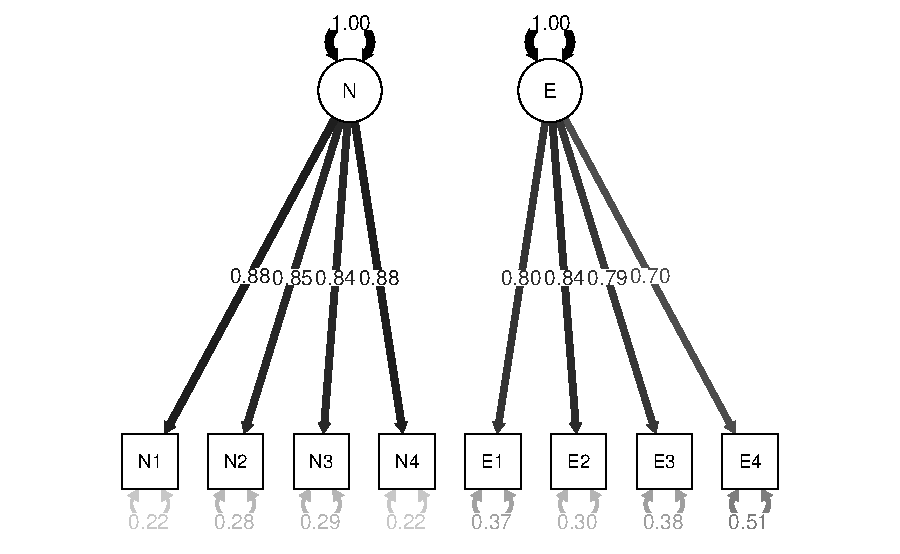
\includegraphics{cfa_book_files/figure-latex/unnamed-chunk-27-1} \end{center}

Come indicato nel diagramma, l'effetto diretto di \texttt{mom\_iq} su \texttt{kid\_score} è identico al corrispondente coefficiente parziale di regressione.

\hypertarget{errore-di-specificazione}{%
\subsection{Errore di specificazione}\label{errore-di-specificazione}}

Spiritosamente chiamato ``heartbreak of L.O.V.E.'' (Left-Out Variable Error; \citet{mauro1990understanding}), l'errore di specificazione è una caratteristica fondamentale dei modelli di regressione che deve sempre essere tenuta a mente quando interpretiamo i risultati di questa analisi statistica. L'errore di specificazione si verifica quando escludiamo dal modello di regressione una variabile che

\begin{itemize}
\tightlist
\item
  è associata con altre variabili nel modello,
\item
  ha un effetto diretto sulla \(y\).
\end{itemize}

Come conseguenza dell'errore di specificazione, la direzione e il segno dei coefficienti parziali di regressione risultano sistematicamente distorti.

Consideriamo un esempio con dati simulati nei quali immaginiamo che la prestazione sia positivamente associata alla motivazione e negativamente associata all'ansia. Immaginiamo inoltre che vi sia una correlazione positiva tra ansia a motivazione. Ci chiediamo cosa succede al coefficiente parziale della variabile ``motivazione'' se la variabile ``ansia'' viene esclusa dal modello di regressione.

\begin{Shaded}
\begin{Highlighting}[]
\FunctionTok{set.seed}\NormalTok{(}\DecValTok{123}\NormalTok{)}
\NormalTok{n }\OtherTok{\textless{}{-}} \DecValTok{400}
\NormalTok{anxiety }\OtherTok{\textless{}{-}} \FunctionTok{rnorm}\NormalTok{(n, }\DecValTok{10}\NormalTok{, }\FloatTok{1.5}\NormalTok{)}
\NormalTok{motivation }\OtherTok{\textless{}{-}} \FloatTok{4.0} \SpecialCharTok{*}\NormalTok{ anxiety }\SpecialCharTok{+} \FunctionTok{rnorm}\NormalTok{(n, }\DecValTok{0}\NormalTok{, }\FloatTok{3.5}\NormalTok{)}
\FunctionTok{cor}\NormalTok{(anxiety, motivation)}
\CommentTok{\#\textgreater{} [1] 0.8618}
\end{Highlighting}
\end{Shaded}

\begin{Shaded}
\begin{Highlighting}[]
\NormalTok{performance }\OtherTok{\textless{}{-}} \FloatTok{0.5} \SpecialCharTok{*}\NormalTok{ motivation }\SpecialCharTok{{-}} \FloatTok{5.0} \SpecialCharTok{*}\NormalTok{ anxiety }\SpecialCharTok{+} \FunctionTok{rnorm}\NormalTok{(n, }\DecValTok{0}\NormalTok{, }\DecValTok{3}\NormalTok{)}
\end{Highlighting}
\end{Shaded}

\begin{Shaded}
\begin{Highlighting}[]
\NormalTok{sim\_dat2 }\OtherTok{\textless{}{-}} \FunctionTok{tibble}\NormalTok{(performance, motivation, anxiety)}
\NormalTok{fm1 }\OtherTok{\textless{}{-}} \FunctionTok{lm}\NormalTok{(performance }\SpecialCharTok{\textasciitilde{}}\NormalTok{ motivation }\SpecialCharTok{+}\NormalTok{ anxiety, sim\_dat2)}
\FunctionTok{coef}\NormalTok{(fm1)}
\CommentTok{\#\textgreater{} (Intercept)  motivation     anxiety }
\CommentTok{\#\textgreater{}      1.3712      0.4954     {-}5.1052}
\end{Highlighting}
\end{Shaded}

\begin{Shaded}
\begin{Highlighting}[]
\NormalTok{fm2 }\OtherTok{\textless{}{-}} \FunctionTok{lm}\NormalTok{(performance }\SpecialCharTok{\textasciitilde{}}\NormalTok{ motivation, sim\_dat2)}
\FunctionTok{summary}\NormalTok{(fm2)}
\CommentTok{\#\textgreater{} }
\CommentTok{\#\textgreater{} Call:}
\CommentTok{\#\textgreater{} lm(formula = performance \textasciitilde{} motivation, data = sim\_dat2)}
\CommentTok{\#\textgreater{} }
\CommentTok{\#\textgreater{} Residuals:}
\CommentTok{\#\textgreater{}     Min      1Q  Median      3Q     Max }
\CommentTok{\#\textgreater{} {-}13.501  {-}3.409   0.005   3.311  12.616 }
\CommentTok{\#\textgreater{} }
\CommentTok{\#\textgreater{} Coefficients:}
\CommentTok{\#\textgreater{}             Estimate Std. Error t value Pr(\textgreater{}|t|)    }
\CommentTok{\#\textgreater{} (Intercept) {-}12.3972     1.4459   {-}8.57  2.2e{-}16 ***}
\CommentTok{\#\textgreater{} motivation   {-}0.4372     0.0355  {-}12.31  \textless{} 2e{-}16 ***}
\CommentTok{\#\textgreater{} {-}{-}{-}}
\CommentTok{\#\textgreater{} Signif. codes:  }
\CommentTok{\#\textgreater{} 0 \textquotesingle{}***\textquotesingle{} 0.001 \textquotesingle{}**\textquotesingle{} 0.01 \textquotesingle{}*\textquotesingle{} 0.05 \textquotesingle{}.\textquotesingle{} 0.1 \textquotesingle{} \textquotesingle{} 1}
\CommentTok{\#\textgreater{} }
\CommentTok{\#\textgreater{} Residual standard error: 4.87 on 398 degrees of freedom}
\CommentTok{\#\textgreater{} Multiple R{-}squared:  0.276,  Adjusted R{-}squared:  0.274 }
\CommentTok{\#\textgreater{} F{-}statistic:  151 on 1 and 398 DF,  p{-}value: \textless{}2e{-}16}
\end{Highlighting}
\end{Shaded}

Il risultato prodotto dal modello di regressione è sbagliato: come conseguenza dell'errore di specificazione, il segno del coefficiente parziale di regressione della variabile ``motivazione'' è negativo, anche se nel vero modello di regressione tale coefficiente ha il segno opposto. Quindi, se noi interpretassimo il coefficiente parziale ottenuto in termini casuali, saremmo portati a concludere che la motivazione fa diminuire la prestazione anche se, in realtà (nel modello generatore dei dati), è vero l'opposto.

È facile vedere perché questo si verifica. Supponiamo che il vero modello sia

\[
y = \alpha + \beta_1 X_1 + \beta_2 X_2 + \varepsilon
\] che verrebbe stimato con

\[
y = a + b_1 X_1 + b_2 X_2 + e.
\] Supponiamo che il ricercatore creda invece che

\[
y = \alpha^\prime + \beta_1^\prime X_1 + \varepsilon^\prime
\]

e quindi stimi

\[
y = a^\prime + b_1^\prime X_1 + e^\prime
\]

omettendo \(X_2\) dal modello. Ci chiediamo che relazione ci sia tra \(b_1^\prime\) e \(b_1\).

La formula per \(b_1^\prime\) è

\begin{equation}
\begin{aligned}
b_1^\prime &= \frac{\mbox{Cov}(X_1, Y)}{\mbox{Var}(X_1)}\notag\\
&= \frac{\mbox{Cov}(X_1, a + b_1 X_1 + b_2 X_2 + e)}{\mbox{Var}(X_1)}\notag\\
&= \frac{\mbox{Cov}(X_1, a)+b_1 \mbox{Cov}(X_1, X_1) + b_2 \mbox{Cov}(X_1, X_2) + \mbox{Cov}(X_1, e)}{\mbox{Var}(X_1)}\notag\\
&= \frac{0 + b_1 \mbox{Var}(X_1) + b_2 \mbox{Cov}(X_1, X_2) + 0}{\mbox{Var}(X_1)}\notag\\
&= b_1 + b_2 \frac{\mbox{Cov}(X_1, X_2)}{\mbox{Var}(X_1)}.
\end{aligned}
\end{equation}

Quindi, se \(X_2\) viene erroneamente omesso dal modello, abbiamo che

\[
\mathbb{E}(b_1^\prime) = \beta_1 + \beta_2 \frac{\sigma_{12}}{\sigma_1^2}.
\] Verifichiamo per i dati dell'esempio che stiamo discutendo. Nel caso presente, \(X_1\) è \texttt{motivation} e \(X_2\) + \texttt{anxiety}. Dunque, applicando la formula precedente, otteniamo lo stesso valore per il coefficiente di regressione associato a \texttt{motivation} che era stato ottenuto adattando ai dati il modello \texttt{performance\ \textasciitilde{}\ motivation}, ovvero:

\begin{Shaded}
\begin{Highlighting}[]
\NormalTok{fm1}\SpecialCharTok{$}\NormalTok{coef[}\DecValTok{2}\NormalTok{] }\SpecialCharTok{+}\NormalTok{ fm1}\SpecialCharTok{$}\NormalTok{coef[}\DecValTok{3}\NormalTok{] }\SpecialCharTok{*}
  \FunctionTok{cov}\NormalTok{(sim\_dat2}\SpecialCharTok{$}\NormalTok{motivation, sim\_dat2}\SpecialCharTok{$}\NormalTok{anxiety) }\SpecialCharTok{/}
  \FunctionTok{var}\NormalTok{(sim\_dat2}\SpecialCharTok{$}\NormalTok{motivation)}
\CommentTok{\#\textgreater{} motivation }
\CommentTok{\#\textgreater{}    {-}0.4372}
\end{Highlighting}
\end{Shaded}

In conclusione, \(b_1^\prime\) è uno stimatore distorto di \(\beta_1\). Si noti che questa distorsione non scomparirà all'aumentare della numerosità campionaria, il che (in termini statistici) ci porta a concludere che un tale stimatore è \emph{inconsistente}. Quello che succede in pratica è che alla variabile \(X_1\) vengono attribuiti gli effetti delle variabili che sono state omesse dal modello. Si noti che una tale distorsione sistematica di \(b_1^\prime\) può essere evitata solo se si verificano due condizioni:

\begin{itemize}
\tightlist
\item
  \(\beta_2 = 0\). Questo è ovvio, dato che, se \(\beta_2 = 0\), ciò significa che il modello non è specificato in modo errato, cioè \(X_2\) non appartiene al modello perché non ha un effetto diretto sulla \(Y\).
\item
  \(\sigma_{12} = 0\). Cioè, se \(X_1\) e \(X_2\) sono incorrelate, allora l'omissione di una delle due variabili non comporta stime distorte dell'effetto dell'altra.
\end{itemize}

\hypertarget{soppressione}{%
\subsection{Soppressione}\label{soppressione}}

Le conseguenze dell'errore di specificazione sono chiamate ``soppressione'' (\emph{suppression}). In generale, si ha soppressione quando (1) il valore assoluto del peso beta di un predittore è maggiore di quello della sua correlazione bivariata con il criterio o (2) i due hanno segni opposti.

\begin{itemize}
\tightlist
\item
  L'esempio descritto sopra è un caso di \emph{soppressione negativa}, dove il predittore ha correlazioni bivariate positive con il criterio, ma si riceve un peso beta negativo nell'analisi di regressione multipla.
\item
  Un secondo tipo di soppressione è la \emph{soppressione classica}, in cui un predittore non è correlato al criterio ma riceve un peso beta diverso da zero se un altro predittore viene controllato.
\item
  C'è anche la \emph{soppressione reciproca} che può verificarsi quando due variabili sono correlate positivamente con il criterio ma negativamente tra loro.
\end{itemize}

\hypertarget{stepwise-regression}{%
\subsection{Stepwise regression}\label{stepwise-regression}}

Un'implicazione della soppressione è che i predittori non dovrebbero essere selezionati in base ai valori delle correlazioni bivariate con il criterio. Queste associazioni di ordine zero non controllano gli effetti degli altri predittori, quindi i loro valori possono essere fuorvianti rispetto ai coefficienti di regressione parziale per le stesse variabili. Per lo stesso motivo, il fatto che le correlazioni bivariate con il criterio siano statisticamente significative o meno è irrilevante per quanto riguarda la selezione dei predittori. Sebbene le procedure informatiche di regressione rendano facile tali processi di selezione dei predittori, i ricercatori dovrebbero evitare di usare tali metodi. Il rischio è che anche piccole, ma non rilevate, non-linearità o effetti indiretti tra i predittori possano seriamente distocere i coefficienti di regressione parziale. È meglio selezionare giudiziosamente il minor numero di predittori sulla base di ragioni teoriche o dei risultati di ricerche precedenti.

Una volta selezionati, ci sono due modi di base per inserire i predittori nell'equazione di regressione: uno consiste nell'inserire tutti i predittori contemporaneamente. L'altro è inserirli nel corso di una serie di passaggi, ovvero mediante usando una procedura sequenziale. L'ordine di ingresso può essere determinato in base a uno di due diversi standard: teorici (razionali) o empirici (statistici). Lo standard razionale corrisponde alla regressione gerarchica, in cui si comunica al computer un ordine fisso per inserire i predittori. Ad esempio, a volte le variabili demografiche vengono inserite nel primo passaggio, quindi nel secondo passaggio viene inserita una variabile psicologica di interesse. Questo ordine non solo controlla le variabili demografiche ma permette anche di valutare il potere predittivo della variabile psicologica, al di là di quello delle semplici variabili demografiche. Quest'ultimo può essere stimato come l'aumento della correlazione multipla al quadrato, o \(\Delta R^2\), da quella della fase 1 con solo predittori demografici a quella della fase 2 con tutti i predittori nell'equazione di regressione.

Un esempio di standard statistico è la regressione \emph{stepwise}, in cui il computer seleziona l'inserimento dei predittori in base esclusivamente alla significatività statistica; cioè, viene chiesto: quale predittore, se inserito nell'equazione, avrebbe il valore\_\(p\) più piccolo per il test del suo coefficiente di regressione parziale? Dopo la selezione, i predittori in una fase successiva possono essere rimossi dall'equazione di regressione in base ai loro valori-\(p\) (ad esempio, se \(p \geq\) .05). Il processo stepwise si interrompe quando, aggiungendo più predittori, \(\Delta R^2\) non migliora. Varianti della regressione stepwise includono \emph{forward inclusion}, in cui i predittori selezionati non vengono successivamente rimossi dal modello, e \emph{backward elimination}, che inizia con tutti i predittori nel modello per poi rimuoverne alcuni in passi successivi. I problemi relativi ai metodi stepwise sono così gravi da essere effettivamente banditi in alcuni giornali. Un problema è che fanno leva su risultati che si ottengono per caso, in dipendenza delle idiosincrasie del campione (quindi, non replicabili).

In secondo luogo, una volta che un insieme finale di predittori selezionati razionalmente è stato inserito nell'equazione di regressione, tali predittori non dovrebbero essere successivamente rimossi se i loro coefficienti di regressione non sono statisticamente significativi: il ricercatore non dovrebbe sentirsi in dovere di lasciar perdere ogni predittore che non risulta statisticamente significativo. In campioni piccoli, la potenza dei test di significatività è bassa e la rimozione di un predittore non significativo può alterare sostanzialmente la soluzione. Se c'è una buona ragione per includere un predittore, allora è meglio lasciarlo nel modello, fino a prova contraria.

\hypertarget{ch:factor-scores}{%
\chapter{I punteggi fattoriali}\label{ch:factor-scores}}

Uno dei momenti più difficili nel processo di sviluppo di un test psicometrico è quello dell'interpretazione dei fattori. La verifica del livello di affidabilità rivela il grado di precisione delle misure ottenute ma non fornisce alcuna informazione sulla natura di ciò che si sta misurando. Non esistono specifiche indicazioni che guidino il lavoro interpretativo. Dipende, perciò, dalla capacità e dall'esperienza del ricercatore cogliere il significato comune delle variabili confluite in un fattore, attenendosi alla realtà delle singole variabili senza fornire interpretazioni fantasiose. È importante rendersi conto che sia la scelta del metodo di estrazione dei fattori, sia il problema del numero dei fattori da estrarre, sia la scelta del metodo con cui effettuare la rotazione, rendono molto arbitraria l'interpretazione della soluzione fattoriale.

I passaggi teorici necessari per interpretare una matrice fattoriale ruotata possono essere descritti nel modo seguente.

\begin{enumerate}
\def\labelenumi{\arabic{enumi}.}
\item
  Si definisce un livello arbitrario per le saturazioni che ci indichi il limite oltre il quale non riteniamo le variabili sufficientemente importanti per caratterizzare quel determinato fattore. Solitamente si sceglie la soglia di .40. In casi particolari è possibile usare valori maggiori o minori di questo, a seconda che si abbia un numero ristretto o troppo ampio di variabili da interpretare.
\item
  Si ordinano le saturazioni delle variabili del fattore in ordine decrescente (in valore assoluto), fermandosi al livello prescelto.
\item
  Si scrive accanto ad ogni saturazione la denominazione della variabile corrispondente (o il testo dell'item).
\item
  Tenendo presente il dominio di indagine, le teorie di riferimento ed eventuali risultati precedenti, si cerca di stabilire quale sia il tratto, caratteristica, aspetto \ldots che queste variabili abbiano in comune, in modo da poter in modo da poter ``nominare'' il fattore che definisce questo tratto comune. In questo processo interpretativo gli item con le saturazioni maggiori contribuiscono in misura maggiore alla definizione del carattere comune del fattore e, viceversa, ciò che è stato individuato come tratto comune delle variabili deve comparire in maggior grado nelle variabili più sature.
\item
  Il segno negativo di una saturazione indica solamente un'opposizione rispetto alle saturazioni positive. Il tratto comune alle variabili dovrebbe essere pensato come un continuum che passa dalla sua massima presenza al suo opposto. Per procedere all'interpretazione conviene iniziare dalle variabili il cui segno è più frequente e considerarle come se fossero positive; di conseguenza, le altre (siano esse di segno positivo o negativo) devono essere considerate di segno opposto.
\item
  Nel caso in cui non si riesca a riscontrare nessun tratto comune alle variabili del fattore, si dovrà concludere che il fattore non è interpretabile e che le variabili sono state tra loro associate per un errore attribuibile o al campione o alla misurazione delle variabili stesse. Normalmente i ``primi'' fattori estratti sono facilmente interpretabili mentre gli ``ultimi'', soprattutto se ne sono stati estratti molti o se la matrice delle correlazioni iniziale fra le variabili contiene molti valori bassi, sono spesso difficilmente interpretabili o saturi di una sola variabile e quindi fattori specifici di quella variabile. In linea di massima se i fattori non interpretabili sono molti è meglio non considerare affatto i risultati dell'analisi fattoriale.
\end{enumerate}

\hypertarget{esempio-di-interpretazione}{%
\subsection{Esempio di interpretazione}\label{esempio-di-interpretazione}}

Il WISC-III (Wechsler Intelligence Scale For Children - III) valuta l'abilità intellettiva di soggetti dai 6 ai 16 anni e 11 mesi. I subtest sono stati selezionati per valutare diverse abilità mentali, che tutte insieme indicano l'abilità intellettiva generale del bambino. Alcuni gli richiedono un ragionamento astratto, altri si focalizzano sulla memoria, altri ancora richiedono certe abilità percettive e così via.

Si consideri la matrice di correlazione tra i subtest della scala WISC-III riportata dal manuale.

\begin{Shaded}
\begin{Highlighting}[]
\NormalTok{lower }\OtherTok{\textless{}{-}} \StringTok{"}
\StringTok{1}
\StringTok{.66      1}
\StringTok{.57 .55      1}
\StringTok{.70 .69 .54       1}
\StringTok{.56 .59 .47 .64      1}
\StringTok{.34 .34 .43 .35 .29      1}
\StringTok{.47 .45 .39 .45 .38 .25      1}
\StringTok{.21 .20 .27 .26 .25 .23 .18      1}
\StringTok{.40 .39 .35 .40 .35 .20 .37 .28      1}
\StringTok{.48 .49 .52 .46 .40 .32 .52 .27 .41      1}
\StringTok{.41 .42 .39 .41 .34 .26 .49 .24 .37 .61      1}
\StringTok{.35 .35 .41 .35 .34 .28 .33 .53 .36 .45 .38      1}
\StringTok{.18 .18 .22 .17 .17 .14 .24 .15 .23 .31 .29 .24     1}
\StringTok{"}
\end{Highlighting}
\end{Shaded}

\begin{Shaded}
\begin{Highlighting}[]
\NormalTok{wisc\_III\_cov }\OtherTok{\textless{}{-}} \FunctionTok{getCov}\NormalTok{(}
\NormalTok{  lower,}
  \AttributeTok{names =} \FunctionTok{c}\NormalTok{(}
    \StringTok{"INFO"}\NormalTok{, }\StringTok{"SIM"}\NormalTok{, }\StringTok{"ARITH"}\NormalTok{, }\StringTok{"VOC"}\NormalTok{, }\StringTok{"COMP"}\NormalTok{, }\StringTok{"DIGIT"}\NormalTok{, }\StringTok{"PICTCOM"}\NormalTok{,}
    \StringTok{"CODING"}\NormalTok{, }\StringTok{"PICTARG"}\NormalTok{, }\StringTok{"BLOCK"}\NormalTok{, }\StringTok{"OBJECT"}\NormalTok{, }\StringTok{"SYMBOL"}\NormalTok{, }\StringTok{"MAZES"}
\NormalTok{  )}
\NormalTok{)}
\end{Highlighting}
\end{Shaded}

Eseguiamo l'analisi fattoriale con il metodo delle componenti principali e una rotazione Varimax:

\begin{Shaded}
\begin{Highlighting}[]
\NormalTok{f\_pc }\OtherTok{\textless{}{-}}\NormalTok{ psych}\SpecialCharTok{::}\FunctionTok{principal}\NormalTok{(wisc\_III\_cov, }\AttributeTok{nfactors =} \DecValTok{3}\NormalTok{, }\AttributeTok{rotate =} \StringTok{"varimax"}\NormalTok{)}
\NormalTok{f\_pc}
\CommentTok{\#\textgreater{} Principal Components Analysis}
\CommentTok{\#\textgreater{} Call: psych::principal(r = wisc\_III\_cov, nfactors = 3, rotate = "varimax")}
\CommentTok{\#\textgreater{} Standardized loadings (pattern matrix) based upon correlation matrix}
\CommentTok{\#\textgreater{}           RC1  RC3  RC2   h2   u2 com}
\CommentTok{\#\textgreater{} INFO     0.80 0.25 0.09 0.72 0.28 1.2}
\CommentTok{\#\textgreater{} SIM      0.81 0.25 0.08 0.72 0.28 1.2}
\CommentTok{\#\textgreater{} ARITH    0.65 0.26 0.28 0.57 0.43 1.7}
\CommentTok{\#\textgreater{} VOC      0.83 0.19 0.13 0.75 0.25 1.2}
\CommentTok{\#\textgreater{} COMP     0.75 0.14 0.16 0.60 0.40 1.2}
\CommentTok{\#\textgreater{} DIGIT    0.45 0.06 0.36 0.34 0.66 2.0}
\CommentTok{\#\textgreater{} PICTCOM  0.43 0.61 0.02 0.56 0.44 1.8}
\CommentTok{\#\textgreater{} CODING   0.10 0.09 0.88 0.79 0.21 1.0}
\CommentTok{\#\textgreater{} PICTARG  0.34 0.45 0.27 0.39 0.61 2.6}
\CommentTok{\#\textgreater{} BLOCK    0.41 0.66 0.22 0.66 0.34 1.9}
\CommentTok{\#\textgreater{} OBJECT   0.31 0.71 0.14 0.62 0.38 1.5}
\CommentTok{\#\textgreater{} SYMBOL   0.23 0.32 0.74 0.70 0.30 1.6}
\CommentTok{\#\textgreater{} MAZES   {-}0.06 0.71 0.11 0.51 0.49 1.1}
\CommentTok{\#\textgreater{} }
\CommentTok{\#\textgreater{}                        RC1  RC3  RC2}
\CommentTok{\#\textgreater{} SS loadings           3.80 2.37 1.74}
\CommentTok{\#\textgreater{} Proportion Var        0.29 0.18 0.13}
\CommentTok{\#\textgreater{} Cumulative Var        0.29 0.47 0.61}
\CommentTok{\#\textgreater{} Proportion Explained  0.48 0.30 0.22}
\CommentTok{\#\textgreater{} Cumulative Proportion 0.48 0.78 1.00}
\CommentTok{\#\textgreater{} }
\CommentTok{\#\textgreater{} Mean item complexity =  1.5}
\CommentTok{\#\textgreater{} Test of the hypothesis that 3 components are sufficient.}
\CommentTok{\#\textgreater{} }
\CommentTok{\#\textgreater{} The root mean square of the residuals (RMSR) is  0.07 }
\CommentTok{\#\textgreater{} }
\CommentTok{\#\textgreater{} Fit based upon off diagonal values = 0.97}
\end{Highlighting}
\end{Shaded}

Si noti che i primi cinque subtest possiedono saturazioni maggiori di \(0.6\) sul primo fattore. Dato che questi test sono tutti presentati verbalmente e richiedono delle risposte verbali, tale fattore può essere denominato \emph{Comprensione Verbale}.

I subtest ``Cifrario'' e ``Ricerca di simboli'' saturano sul secondo fattore. Entrambi i subtest misurano la velocità dei processi di codifica o ricerca. Questo fattore, dunque, può essere denominato \emph{Velocità di elaborazione}.

Infine, i subtest ``Completamento di figure,'' ``Disegno con i cubi,'' ``Riordinamento di storie figurate'' e ``Labirinti'' saturano sul terzo fattore. Tutti questi test condividono una componente geometrica o configurazionale: misurano infatti le abilità necessarie per la manipolazione o la disposizione di immagini, oggetti, blocchi. Questo fattore, dunque, può essere denominato \emph{Organizzazione percettiva}.

Nel caso di una rotazione ortogonale, la comunalità di ciascuna sottoscala è uguale alla somma dei coefficienti di impatto al quadrato della sottoscala nei fattori. Per le 13 sottoscale del WISC-III abbiamo dunque

\begin{Shaded}
\begin{Highlighting}[]
\NormalTok{h2 }\OtherTok{\textless{}{-}} \FunctionTok{rep}\NormalTok{(}\DecValTok{0}\NormalTok{, }\DecValTok{13}\NormalTok{)}
\ControlFlowTok{for}\NormalTok{ (i }\ControlFlowTok{in} \DecValTok{1}\SpecialCharTok{:}\DecValTok{13}\NormalTok{) \{}
\NormalTok{  h2[i] }\OtherTok{\textless{}{-}} \FunctionTok{sum}\NormalTok{(f\_pc}\SpecialCharTok{$}\NormalTok{loadings[i, ]}\SpecialCharTok{\^{}}\DecValTok{2}\NormalTok{)}
\NormalTok{\}}
\FunctionTok{round}\NormalTok{(h2, }\DecValTok{2}\NormalTok{)}
\CommentTok{\#\textgreater{}  [1] 0.72 0.72 0.57 0.75 0.60 0.34 0.56 0.79 0.39 0.66}
\CommentTok{\#\textgreater{} [11] 0.62 0.70 0.51}
\end{Highlighting}
\end{Shaded}

Questi risultati replicano quelli riportati nel manuale del test WISC-III.

\hypertarget{punteggi-fattoriali}{%
\section{Punteggi fattoriali}\label{punteggi-fattoriali}}

Fino ad ora abbiamo considerato le strategie di costruzione del modello basate sulla stima e sull'interpretazione delle saturazioni fattoriali e delle comunalità. Questo è il primo passo nella costruzione del modello fattoriale. È però possibile compiere un passo ulteriore, ovvero quello della stima dei punteggi fattoriali (\emph{factor scores}) i quali risultano utili sia per interpretare i risultati dell'analisi fattoriale che per fare diagnostica. I punteggi fattoriali forniscono le previsioni dei livelli dei fattori latenti per ogni rispondente. Esistono vari metodi di stima dei punteggi fattoriali. Tra questi troviamo il metodo di Thomson basato sulla regressione e il metodo di Bartlett basato sulla massima verosimiglianza. Entrambi questi metodi sono implementati nel software .

\hypertarget{stima-dei-punteggi-fattoriali}{%
\subsection{Stima dei punteggi fattoriali}\label{stima-dei-punteggi-fattoriali}}

Si definiscono punteggi fattoriali i valori assunti dai fattori comuni (inosservabili) in corrispondenza delle osservazioni campionarie. Il metodo di Thomson stima i punteggi fattoriali in base all'approccio della regressione multipla, ovvero, impiegando la matrice delle correlazioni tra le variabili e la matrice di struttura (ovvero, la matrice delle correlazioni delle variabili con i fattori). Per ottenere le stime dei punteggi fattoriali con il metodo di Thomson è necessario specificare nella funzione \texttt{factanal()} l'opzione \texttt{scores\ =\ "regression"}.

\hypertarget{dimostrazione-di-thurstone}{%
\subsection{Dimostrazione di Thurstone}\label{dimostrazione-di-thurstone}}

Prima di descrivere il metodo della regressione, esaminiamo la dimostrazione che Thurstone (1947) ha fornito per illustrare il significato dei punteggi fattoriali (si veda Loehlin, 1987). L'idea è quella di esaminare la stima dei punteggi fattoriali in una situazione in cui i tali punteggi sono conosciuti, in maniera tale da potere controllare il risultato dell'analisi.

Si consideri un insieme di 1000 scatole di cui conosciamo le dimensioni \(x, y, z\):

\begin{Shaded}
\begin{Highlighting}[]
\FunctionTok{set.seed}\NormalTok{(}\DecValTok{123}\NormalTok{)}
\NormalTok{n }\OtherTok{\textless{}{-}} \FloatTok{1e3}
\NormalTok{x }\OtherTok{\textless{}{-}} \FunctionTok{rnorm}\NormalTok{(n, }\DecValTok{100}\NormalTok{, }\FloatTok{1.5}\NormalTok{)}
\NormalTok{y }\OtherTok{\textless{}{-}} \FunctionTok{rnorm}\NormalTok{(n, }\DecValTok{200}\NormalTok{, }\FloatTok{1.5}\NormalTok{)}
\NormalTok{z }\OtherTok{\textless{}{-}} \FunctionTok{rnorm}\NormalTok{(n, }\DecValTok{300}\NormalTok{, }\FloatTok{1.5}\NormalTok{)}
\end{Highlighting}
\end{Shaded}

Il problema è quello di stimare le dimensioni delle scatole disponendo soltanto di una serie di misure indirette, corrotte dal rumore di misura. Thurstone (1947) utilizzò le seguenti trasformazioni delle dimensioni delle scatole (si veda Jennrich, 2007).

\begin{Shaded}
\begin{Highlighting}[]
\NormalTok{s }\OtherTok{\textless{}{-}} \DecValTok{40}
\NormalTok{y1 }\OtherTok{\textless{}{-}} \FunctionTok{rnorm}\NormalTok{(n, }\FunctionTok{mean}\NormalTok{(x), s)}
\NormalTok{y2 }\OtherTok{\textless{}{-}} \FunctionTok{rnorm}\NormalTok{(n, }\FunctionTok{mean}\NormalTok{(y), s)}
\NormalTok{y3 }\OtherTok{\textless{}{-}} \FunctionTok{rnorm}\NormalTok{(n, }\FunctionTok{mean}\NormalTok{(z), s)}
\NormalTok{y4 }\OtherTok{\textless{}{-}}\NormalTok{ x }\SpecialCharTok{*}\NormalTok{ y }\SpecialCharTok{+} \FunctionTok{rnorm}\NormalTok{(n, }\DecValTok{0}\NormalTok{, s)}
\NormalTok{y5 }\OtherTok{\textless{}{-}}\NormalTok{ x }\SpecialCharTok{*}\NormalTok{ z }\SpecialCharTok{+} \FunctionTok{rnorm}\NormalTok{(n, }\DecValTok{0}\NormalTok{, s)}
\NormalTok{y6 }\OtherTok{\textless{}{-}}\NormalTok{ y }\SpecialCharTok{*}\NormalTok{ z }\SpecialCharTok{+} \FunctionTok{rnorm}\NormalTok{(n, }\DecValTok{0}\NormalTok{, s)}
\NormalTok{y7 }\OtherTok{\textless{}{-}}\NormalTok{ x}\SpecialCharTok{\^{}}\DecValTok{2} \SpecialCharTok{*}\NormalTok{ y }\SpecialCharTok{+} \FunctionTok{rnorm}\NormalTok{(n, }\DecValTok{0}\NormalTok{, s)}
\NormalTok{y8 }\OtherTok{\textless{}{-}}\NormalTok{ x }\SpecialCharTok{*}\NormalTok{ y}\SpecialCharTok{\^{}}\DecValTok{2} \SpecialCharTok{+} \FunctionTok{rnorm}\NormalTok{(n, }\DecValTok{0}\NormalTok{, s)}
\NormalTok{y9 }\OtherTok{\textless{}{-}}\NormalTok{ x}\SpecialCharTok{\^{}}\DecValTok{2} \SpecialCharTok{*}\NormalTok{ z }\SpecialCharTok{+} \FunctionTok{rnorm}\NormalTok{(n, }\DecValTok{0}\NormalTok{, s)}
\NormalTok{y10 }\OtherTok{\textless{}{-}}\NormalTok{ x }\SpecialCharTok{*}\NormalTok{ z}\SpecialCharTok{\^{}}\DecValTok{2} \SpecialCharTok{+} \FunctionTok{rnorm}\NormalTok{(n, }\DecValTok{0}\NormalTok{, s)}
\NormalTok{y11 }\OtherTok{\textless{}{-}}\NormalTok{ y}\SpecialCharTok{\^{}}\DecValTok{2} \SpecialCharTok{*}\NormalTok{ z }\SpecialCharTok{+} \FunctionTok{rnorm}\NormalTok{(n, }\DecValTok{0}\NormalTok{, s)}
\NormalTok{y12 }\OtherTok{\textless{}{-}}\NormalTok{ y }\SpecialCharTok{*}\NormalTok{ z}\SpecialCharTok{\^{}}\DecValTok{2} \SpecialCharTok{+} \FunctionTok{rnorm}\NormalTok{(n, }\DecValTok{0}\NormalTok{, s)}
\NormalTok{y13 }\OtherTok{\textless{}{-}}\NormalTok{ y}\SpecialCharTok{\^{}}\DecValTok{2} \SpecialCharTok{*}\NormalTok{ z }\SpecialCharTok{+} \FunctionTok{rnorm}\NormalTok{(n, }\DecValTok{0}\NormalTok{, s)}
\NormalTok{y14 }\OtherTok{\textless{}{-}}\NormalTok{ y }\SpecialCharTok{*}\NormalTok{ z}\SpecialCharTok{\^{}}\DecValTok{2} \SpecialCharTok{+} \FunctionTok{rnorm}\NormalTok{(n, }\DecValTok{0}\NormalTok{, s)}
\NormalTok{y15 }\OtherTok{\textless{}{-}}\NormalTok{ x }\SpecialCharTok{/}\NormalTok{ y }\SpecialCharTok{+} \FunctionTok{rnorm}\NormalTok{(n, }\DecValTok{0}\NormalTok{, s)}
\NormalTok{y16 }\OtherTok{\textless{}{-}}\NormalTok{ y }\SpecialCharTok{/}\NormalTok{ x }\SpecialCharTok{+} \FunctionTok{rnorm}\NormalTok{(n, }\DecValTok{0}\NormalTok{, s)}
\NormalTok{y17 }\OtherTok{\textless{}{-}}\NormalTok{ x }\SpecialCharTok{/}\NormalTok{ z }\SpecialCharTok{+} \FunctionTok{rnorm}\NormalTok{(n, }\DecValTok{0}\NormalTok{, s)}
\NormalTok{y18 }\OtherTok{\textless{}{-}}\NormalTok{ z }\SpecialCharTok{/}\NormalTok{ x }\SpecialCharTok{+} \FunctionTok{rnorm}\NormalTok{(n, }\DecValTok{0}\NormalTok{, s)}
\NormalTok{y19 }\OtherTok{\textless{}{-}}\NormalTok{ y }\SpecialCharTok{/}\NormalTok{ z }\SpecialCharTok{+} \FunctionTok{rnorm}\NormalTok{(n, }\DecValTok{0}\NormalTok{, s)}
\NormalTok{y20 }\OtherTok{\textless{}{-}}\NormalTok{ z }\SpecialCharTok{/}\NormalTok{ y }\SpecialCharTok{+} \FunctionTok{rnorm}\NormalTok{(n, }\DecValTok{0}\NormalTok{, s)}
\NormalTok{y21 }\OtherTok{\textless{}{-}} \DecValTok{2} \SpecialCharTok{*}\NormalTok{ x }\SpecialCharTok{+} \DecValTok{2} \SpecialCharTok{*}\NormalTok{ y }\SpecialCharTok{+} \FunctionTok{rnorm}\NormalTok{(n, }\DecValTok{0}\NormalTok{, s)}
\NormalTok{y22 }\OtherTok{\textless{}{-}} \DecValTok{2} \SpecialCharTok{*}\NormalTok{ x }\SpecialCharTok{+} \DecValTok{2} \SpecialCharTok{*}\NormalTok{ z }\SpecialCharTok{+} \FunctionTok{rnorm}\NormalTok{(n, }\DecValTok{0}\NormalTok{, s)}
\NormalTok{y23 }\OtherTok{\textless{}{-}} \DecValTok{2} \SpecialCharTok{*}\NormalTok{ y }\SpecialCharTok{+} \DecValTok{2} \SpecialCharTok{*}\NormalTok{ z }\SpecialCharTok{+} \FunctionTok{rnorm}\NormalTok{(n, }\DecValTok{0}\NormalTok{, s)}
\end{Highlighting}
\end{Shaded}

Eseguiamo l'analisi fattoriale con una soluzione a tre fattori sui dati così creati.

\begin{Shaded}
\begin{Highlighting}[]
\NormalTok{Y }\OtherTok{\textless{}{-}} \FunctionTok{cbind}\NormalTok{(}
\NormalTok{  y1, y2, y3, y4, y5, y6, y7, y8, y9,}
\NormalTok{  y10, y11, y12, y13, y14, y15, y16,}
\NormalTok{  y17, y18, y19, y20, y21, y22, y23}
\NormalTok{)}

\NormalTok{fa }\OtherTok{\textless{}{-}} \FunctionTok{factanal}\NormalTok{(}
\NormalTok{  Y,}
  \AttributeTok{factors =} \DecValTok{3}\NormalTok{,}
  \AttributeTok{scores =} \StringTok{"regression"}\NormalTok{,}
  \AttributeTok{lower =} \FloatTok{0.01}
\NormalTok{)}
\end{Highlighting}
\end{Shaded}

L'opzione \texttt{scores\ =\ "regression"} richiede il calcolo dei punteggi fattoriali con il metodo della regressione. Nel caso di una rotazione Varimax (default della funzione \texttt{factanal()}), i punteggi fattoriali risultano ovviamente incorrelati:

\begin{Shaded}
\begin{Highlighting}[]
\FunctionTok{cor}\NormalTok{(}
  \FunctionTok{cbind}\NormalTok{(fa}\SpecialCharTok{$}\NormalTok{scores[, }\DecValTok{1}\NormalTok{], fa}\SpecialCharTok{$}\NormalTok{scores[, }\DecValTok{2}\NormalTok{], fa}\SpecialCharTok{$}\NormalTok{scores[, }\DecValTok{3}\NormalTok{])}
\NormalTok{) }\SpecialCharTok{\%\textgreater{}\%}
  \FunctionTok{round}\NormalTok{(}\DecValTok{3}\NormalTok{)}
\CommentTok{\#\textgreater{}        [,1]  [,2]   [,3]}
\CommentTok{\#\textgreater{} [1,]  1.000 0.002 {-}0.001}
\CommentTok{\#\textgreater{} [2,]  0.002 1.000  0.005}
\CommentTok{\#\textgreater{} [3,] {-}0.001 0.005  1.000}
\end{Highlighting}
\end{Shaded}

Generiamo ora i diagrammi di dispersione che mettono in relazione le dimensioni originarie delle scatole (\(x, y, z\)) con i punteggi fattoriali sui tre fattori. Se l'analisi ha successo, ci aspettiamo un'alta correlazione tra i punteggi fattoriali di ogni fattore e una sola delle dimensioni delle scatole \(x\), \(y\), \(z\).

\begin{Shaded}
\begin{Highlighting}[]
\NormalTok{p1 }\OtherTok{\textless{}{-}} \FunctionTok{tibble}\NormalTok{(x, }\AttributeTok{fs1 =}\NormalTok{ fa}\SpecialCharTok{$}\NormalTok{scores[, }\DecValTok{1}\NormalTok{]) }\SpecialCharTok{\%\textgreater{}\%}
  \FunctionTok{ggplot}\NormalTok{(}\FunctionTok{aes}\NormalTok{(x, fs1)) }\SpecialCharTok{+}
  \FunctionTok{geom\_point}\NormalTok{(}\AttributeTok{alpha =} \FloatTok{0.2}\NormalTok{)}
\NormalTok{p2 }\OtherTok{\textless{}{-}} \FunctionTok{tibble}\NormalTok{(y, }\AttributeTok{fs1 =}\NormalTok{ fa}\SpecialCharTok{$}\NormalTok{scores[, }\DecValTok{1}\NormalTok{]) }\SpecialCharTok{\%\textgreater{}\%}
  \FunctionTok{ggplot}\NormalTok{(}\FunctionTok{aes}\NormalTok{(y, fs1)) }\SpecialCharTok{+}
  \FunctionTok{geom\_point}\NormalTok{(}\AttributeTok{alpha =} \FloatTok{0.2}\NormalTok{)}
\NormalTok{p3 }\OtherTok{\textless{}{-}} \FunctionTok{tibble}\NormalTok{(z, }\AttributeTok{fs1 =}\NormalTok{ fa}\SpecialCharTok{$}\NormalTok{scores[, }\DecValTok{1}\NormalTok{]) }\SpecialCharTok{\%\textgreater{}\%}
  \FunctionTok{ggplot}\NormalTok{(}\FunctionTok{aes}\NormalTok{(z, fs1)) }\SpecialCharTok{+}
  \FunctionTok{geom\_point}\NormalTok{(}\AttributeTok{alpha =} \FloatTok{0.2}\NormalTok{)}

\NormalTok{p4 }\OtherTok{\textless{}{-}} \FunctionTok{tibble}\NormalTok{(x, }\AttributeTok{fs2 =}\NormalTok{ fa}\SpecialCharTok{$}\NormalTok{scores[, }\DecValTok{2}\NormalTok{]) }\SpecialCharTok{\%\textgreater{}\%}
  \FunctionTok{ggplot}\NormalTok{(}\FunctionTok{aes}\NormalTok{(x, fs2)) }\SpecialCharTok{+}
  \FunctionTok{geom\_point}\NormalTok{(}\AttributeTok{alpha =} \FloatTok{0.2}\NormalTok{)}
\NormalTok{p5 }\OtherTok{\textless{}{-}} \FunctionTok{tibble}\NormalTok{(y, }\AttributeTok{fs2 =}\NormalTok{ fa}\SpecialCharTok{$}\NormalTok{scores[, }\DecValTok{2}\NormalTok{]) }\SpecialCharTok{\%\textgreater{}\%}
  \FunctionTok{ggplot}\NormalTok{(}\FunctionTok{aes}\NormalTok{(y, fs2)) }\SpecialCharTok{+}
  \FunctionTok{geom\_point}\NormalTok{(}\AttributeTok{alpha =} \FloatTok{0.2}\NormalTok{)}
\NormalTok{p6 }\OtherTok{\textless{}{-}} \FunctionTok{tibble}\NormalTok{(z, }\AttributeTok{fs2 =}\NormalTok{ fa}\SpecialCharTok{$}\NormalTok{scores[, }\DecValTok{2}\NormalTok{]) }\SpecialCharTok{\%\textgreater{}\%}
  \FunctionTok{ggplot}\NormalTok{(}\FunctionTok{aes}\NormalTok{(z, fs2)) }\SpecialCharTok{+}
  \FunctionTok{geom\_point}\NormalTok{(}\AttributeTok{alpha =} \FloatTok{0.2}\NormalTok{)}

\NormalTok{p7 }\OtherTok{\textless{}{-}} \FunctionTok{tibble}\NormalTok{(x, }\AttributeTok{fs3 =}\NormalTok{ fa}\SpecialCharTok{$}\NormalTok{scores[, }\DecValTok{3}\NormalTok{]) }\SpecialCharTok{\%\textgreater{}\%}
  \FunctionTok{ggplot}\NormalTok{(}\FunctionTok{aes}\NormalTok{(x, fs3)) }\SpecialCharTok{+}
  \FunctionTok{geom\_point}\NormalTok{(}\AttributeTok{alpha =} \FloatTok{0.2}\NormalTok{)}
\NormalTok{p8 }\OtherTok{\textless{}{-}} \FunctionTok{tibble}\NormalTok{(y, }\AttributeTok{fs3 =}\NormalTok{ fa}\SpecialCharTok{$}\NormalTok{scores[, }\DecValTok{3}\NormalTok{]) }\SpecialCharTok{\%\textgreater{}\%}
  \FunctionTok{ggplot}\NormalTok{(}\FunctionTok{aes}\NormalTok{(y, fs3)) }\SpecialCharTok{+}
  \FunctionTok{geom\_point}\NormalTok{(}\AttributeTok{alpha =} \FloatTok{0.2}\NormalTok{)}
\NormalTok{p9 }\OtherTok{\textless{}{-}} \FunctionTok{tibble}\NormalTok{(z, }\AttributeTok{fs3 =}\NormalTok{ fa}\SpecialCharTok{$}\NormalTok{scores[, }\DecValTok{3}\NormalTok{]) }\SpecialCharTok{\%\textgreater{}\%}
  \FunctionTok{ggplot}\NormalTok{(}\FunctionTok{aes}\NormalTok{(z, fs3)) }\SpecialCharTok{+}
  \FunctionTok{geom\_point}\NormalTok{(}\AttributeTok{alpha =} \FloatTok{0.2}\NormalTok{)}
\end{Highlighting}
\end{Shaded}

\begin{Shaded}
\begin{Highlighting}[]
\NormalTok{(p1 }\SpecialCharTok{|}\NormalTok{ p2 }\SpecialCharTok{|}\NormalTok{ p3) }\SpecialCharTok{/}
\NormalTok{  (p4 }\SpecialCharTok{|}\NormalTok{ p5 }\SpecialCharTok{|}\NormalTok{ p6) }\SpecialCharTok{/}
\NormalTok{  (p7 }\SpecialCharTok{|}\NormalTok{ p8 }\SpecialCharTok{|}\NormalTok{ p9)}
\end{Highlighting}
\end{Shaded}

\begin{center}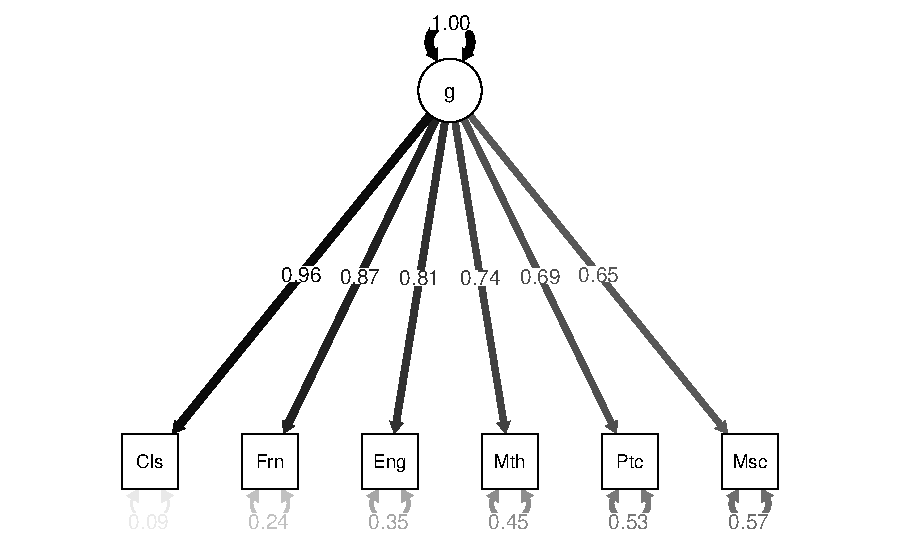
\includegraphics{cfa_book_files/figure-latex/unnamed-chunk-43-1} \end{center}

I risultati riportati nella figura confermano le aspettative.

Il metodo della regressione pone il problema della stima dei punteggi fattoriali nei termini di una ideale regressione di ogni fattore rispetto a tutte le variabili osservate. Per il fattore \(j\)-esimo, si può scrivere la seguente equazione:

\[
\begin{aligned}
F_j =& \beta_{1j}y_1 + \dots + \beta_{pm}y_p + \varepsilon_j
\end{aligned}
\]

dove \(F_j\) sono i punteggi fattoriali e \(y\) sono le variabili osservate standardizzate \((Y-\bar{Y})/s\). In forma matriciale, il modello diventa

\[
\textbf{F} = \textbf{y} \textbf{B} +
\boldsymbol{\varepsilon}
\]

I coefficienti parziali di regressione \textbf{B} sono ignoti. Tuttavia, possono essere calcolati utilizzando i metodi della regressione lineare. Nel modello di regressione, infatti, i coefficienti dei minimi quadrati possono essere calcolati utilizzando due matrici di correlazioni: la matrice \(\textbf{R}_{xx}\) (le correlazioni tra le variabili \(X\)) e la matrice \(\textbf{R}_{xy}\) (le correlazioni tra le variabili \(X\) e la variabile \(Y\):

\[
\hat{\textbf{B}} = \textbf{R}_{xx}^{-1}\textbf{R}_{xy}
\]

Nel caso dell'analisi fattoriale, \(\textbf{R}_{xx}\) corrisponde alla matrice delle correlazioni tra le variabili osservate e \(\textbf{R}_{xy}\) corrisponde alla matrice di struttura (la matrice delle correlazioni tra le variabili osservate e i fattori). Se i fattori sono ortogonali, la matrice di struttura coincide con la matrice dei pesi fattoriali \(\hat{\boldsymbol{\Lambda}}\).

I coefficienti \textbf{B} dell'equazione precedente possono dunque essere trovati nel modo seguente:

\begin{equation}
\hat{\textbf{B}} = \textbf{R}_{yy}^{-1}\textbf{R}_{xf}=
\textbf{R}^{-1}\hat{\boldsymbol{\Lambda}}
\end{equation}

Una volta stimati i coefficienti \(\hat{\textbf{B}}\), i punteggi fattoriali si calcolano allo stesso modo dei punteggi teorici del modello di regressione:

\begin{equation}
\hat{\textbf{F}} = \textbf{y} \hat{\textbf{B}} = \textbf{y}
\textbf{R}^{-1}\hat{\boldsymbol{\Lambda}},
\end{equation}

dove \(\textbf{y}\) è la matrice delle variabili osservate standardizzate \((Y-\bar{Y})/s\).

  \bibliography{refs.bib,book.bib,packages.bib}

\printindex

\end{document}
